% Chapter Template

\chapter{Security} % Main chapter title

\label{Chapter: Security} % Change X to a consecutive number; for referencing this chapter elsewhere, use \ref{ChapterX}

\lhead{Chapter 5. \emph{Security in Petri nets}} % Change X to a consecutive number; this is for the header on each page - perhaps a shortened title

%----------------------------------------------------------------------------------------
%       SECURITY
%----------------------------------------------------------------------------------------
%----------------------------------------------------------------------------------------
%       SECURITY: Introduction
%----------------------------------------------------------------------------------------
\section{Introduction}

This is the second main goal, after subnetting. Once the possible subnets are defined it is the turn of securing them. It is possible to secure Petri subnets or the entire net.

With secure, I mean four goals:
\begin{itemize}
\item \textbf{Privacy}. Concrete parts of the net must be occulted: the content is secret, so not everybody should be able to know it.
\item \textbf{Integrity}. Any change in the secured parts has to be detected.
If any of these parts suffers any kind of modification, the information may have been compromised,
and perhaps it is not valid or correct. But I cannot know what has been modified:
I can only detect that the original content has been changed.
\item \textbf{Authentication}. I can authenticate the source of that net/subnet (the signer,
author or guarantor).
\item \textbf{Non repudiation}. With this characteristic, the possibility of supplant other people is avoided. So the person that signs that part cannot
say that he hadn't done it. The signer cannot deny  it. 

\end{itemize}

There can be several reasons for hiding information of a Petri net. For example:

\begin{itemize}
\item One subnet is a secret process that I want to hide from indiscrete
eyes
\item I have a main process that communicates with other processes. These
processes are susceptible to be changed and the only information I need is
the interface, so they can be easily replaced by other implementations.
\end{itemize}

But this information should be accessible to authorized
people without necessity of supplying any other kind of data.
So the whole information may be stored in the same file.

In the same way, there can be many reasons for the rest of the security characteristics.
For example, suppose that we have a Petri net that several people can access
and:
\begin{itemize}
\item Some parts of that Petri net have been validated an accepted, so I
want nobody to change them. In this case  \textbf{integrity} is needed.
\item I want to know who has developed a concrete chunk of the net. \textbf{Authentication}
is required.

\item There is a part of the Petri net that is bad defined and goes wrong.
The person responsible of this part says that he hasn't made it and somebody has
supplanted him. Then, \textbf{non repudiation} is needed.
\end{itemize}



The best way to reach these goals is using standard and proved
technologies. In this case, the selected technologies are: 
\begin{itemize}
\item XMLEncryption\cite{XMLENC-w3.org/xmlenc-core1} for privacy.
\item XMLSignature \cite{XMLSIG-w3.org/xmlsig-core1} for integrity, authentication and non repudiation.
\end{itemize}


%----------------------------------------------------------------------------------------
%       SECURITY: XMLEncryption
%----------------------------------------------------------------------------------------

\section{XMLEncryption}


\subsection{XMLEncryption revision}
XMLEncryption is a World Wide Web Consortium (W3C)
Recommendation for  encrypting xml or non xml content. It is a standard
xml file cipher. Both symmetric and asymmetric ciphering can be used, but in this case, symmetric is preferred.
The main idea of this encryption is to replace the xml element or elements
we want to be ciphered by other xml code that contains the ciphered data, in addition to information of the algorithms and keys used for the encryption process. When a non xml file is ciphered, the only option is to encrypt it completely. But,  when it is applied to xml content, this technology allows us to define concrete fragments of the document we want to hide. Moreover, the xml document can be transformed before applying the encryption, for example, in order to normalize the xml content.
In this work, the pieces of xml content susceptible to be ciphered are, obviously,
the subnets represented in PNML format. 

Regardless of the data source (xml or non xml) the result is always a xml element. Normal is that this xml encrypted chunk has the whole necessary information to be decrypted. Among that information we can find:

\begin{itemize}
\item Ciphering algorithm: it is the name of chosen method to encrypt
the data. It can be not included. In this case, both ciphering and deciphering agents have to know which is the exact this algorithm.
\item The ciphered data: obviously this part is mandatory and has always
to be present.
\item Name of the chosen key: it is optional. It is used when a set of keys is known by both ciphering and deciphering agents.
\item Key: it is optional. In this case there is a symmetric key in order
to encrypt the data and an additional pair of keys: one (known by the cipher
agent) to encrypt the symmetric key and the other (known by the decipher agent) to decrypt it. 
\end{itemize} 

Actually, there are several options to apply XMLEncryption, such as the algorithm
or the key. The exact election of those option values is responsibility of the Petri net sender. For example:
\begin{itemize}
 \item Maybe both parts (sender and receiver) have a common
set of keys, so they can use it in order to encrypt and decrypt the subnet
content.
 \item Other common use is that
the key is defined inside the options but it is ciphered itself. If the receiver
have a pair of keys (public and private) and an asymmetrical algorithm (such as Diffie-Hellman or RSA) , the symmetric key can be ciphered by
the sender with the receiver's public key. In this case, only the receiver
can decrypt it using his private key.
\end{itemize}

This section does not want to be an extensive explanation about XMLEncryption
but a general idea about its functionality. So I am not going to deepen the
whole characteristics of XMLEncryption. The final decision about which options
use is responsibility of those people that want to apply this work, basing their decision on the requirements of their own Petri net. 
 
Once this is said, here we have a basic example of XMLEncryption. Let's take this original xml document:

\begin{lstlisting}[label=xmlenc_example_1_1,caption=Clear xml content]
<?xml version='1.0'?>
<PaymentInfo xmlns='http://example.org/paymentv2'>
  <Name>John Smith</Name>
  <CreditCard Limit='5,000' Currency='USD'>
    <Number>4019 2445 0277 5567</Number>
    <Issuer>Example Bank</Issuer>
    <Expiration>04/02</Expiration>
  </CreditCard>
</PaymentInfo>
\end{lstlisting}

In this example, we want to hide the credit card number \texttt{\textless Number\textgreater}. Several options are going to be applied: with and without
the ciphering information


First of all let's see which will be the aspect of the ciphered content without
information about ciphering, only replacing the clear data by the encrypted
data:
we have not information about  the key or the ciphering algorithm. This
is the xml ciphered code:
\begin{lstlisting}[label=xmlenc_example_1_2,caption=Ciphered xml content
without ciphering information]
<?xml version='1.0'?>
<PaymentInfo xmlns='http://example.org/paymentv2'>
  <Name>John Smith</Name>
  <CreditCard Limit='5,000' Currency='USD'>
    <Number>
      <xenc:EncryptedData xmlns='http://www.w3.org/2001/04/xmlenc#'
          Type='http://www.w3.org/2001/04/xmlenc#Content'>
        <xenc:CipherData>
          <xenc:CipherValue>A23B45C56</CipherValue>
        </CipherData>
      </EncryptedData>
    </Number>
    <Issuer>Example Bank</Issuer>
    <Expiration>04/02</Expiration>
  </CreditCard>
</PaymentInfo>
\end{lstlisting}

As we can see, the credit card number has been replaced by a new 
tag \texttt{\textless EncryptedData\textgreater} that contains the ciphered credit card number.

\note{A new namespace \texttt{xenc} appear  that is the standard namespace
for XMLEncryption. However, in further examples this namespace can be delete
for clarity and for space problems without loss of generality.}

And now let's see how does this same example with information about the algorithm:

\begin{lstlisting}[label=xmlenc_example_1_3,caption=Ciphered xml content
with algorithm information]
<?xml version='1.0'?>
<PaymentInfo xmlns='http://example.org/paymentv2'>
  <Name>John Smith</Name>
  <CreditCard Limit='5,000' Currency='USD'>
    <Number>
      <xenc:EncryptedData xmlns='http://www.w3.org/2001/04/xmlenc#'
          Type='http://www.w3.org/2001/04/xmlenc#Content'>
        <xenc:EncryptionMethod  
            Algorithm="http://www.w3.org/2001/04/xmlenc#aes128-cbc"  
            xmlns:xenc="http://www.w3.org/2001/04/xmlenc#" />  
        <xenc:CipherData>
          <xenc:CipherValue>A23B45C56</CipherValue>
        </CipherData>
      </EncryptedData>
    </Number>
    <Issuer>Example Bank</Issuer>
    <Expiration>04/02</Expiration>
  </CreditCard>
</PaymentInfo>
\end{lstlisting}

As we can see, a new tag \texttt{\textless EncryptedMethod\textgreater}\ has
appeared
inside the \texttt{\textless EncryptedData\textgreater} tag with the algorithm used to cipher. In this case
is \texttt{aes128-cbc}. 

There is other method of Encryption that cipher the tag too. In this case,
we would have the next code:

\begin{lstlisting}[label=xmlenc_example_1_4,caption=Ciphered xml content
including the tag itself]
<?xml version='1.0'?>
<PaymentInfo xmlns='http://example.org/paymentv2'>
  <Name>John Smith</Name>
  <CreditCard Limit='5,000' Currency='USD'>
    <xenc:EncryptedData xmlns='http://www.w3.org/2001/04/xmlenc#'
        Type='http://www.w3.org/2001/04/xmlenc#Element'>
      <xenc:EncryptionMethod  
          Algorithm="http://www.w3.org/2001/04/xmlenc#aes128-cbc"  
          xmlns:xenc="http://www.w3.org/2001/04/xmlenc#" />  
      <xenc:CipherData>
        <xenc:CipherValue>A223B3B493G5C569M</CipherValue>
      </CipherData>
    </EncryptedData>
    <Issuer>Example Bank</Issuer>
    <Expiration>04/02</Expiration>
  </CreditCard>
</PaymentInfo>
\end{lstlisting}

As we can see, the tag \texttt{\textless Number\textgreater} 
has disappeared and it has been included into the \texttt{\textless CipherValue\textgreater}
of the \texttt{\textless CipherData\textgreater}.

 

This is a little approach to XMLEncryption functionality, but enough for
understanding the next section.


\subsection{XMLEncryption and Petri nets}

Once described XMLEncryption it is time to apply it in order to hide part
of a Petri net. Remembering the chapter \ref{Chapter: PNML}, we have one Petri net with one or more subnets represented in a PNML file. These subnets are represented by a \texttt{<subnet>} tag that contains \texttt{<interface>} and
\texttt{<content>}. This last tag contains the
xml content that is going to be ciphered. Obviously, if we encrypt the interface
we will have no way to connect the subnet with the rest of the net.

Let's take back the example used to explain the process of subnetting in
the figure \ref{fig:PNML_SubredEjemplo1}...

\[
\includegraphics[width=0.60\textwidth]{Figures/PNML-SubredEjemplo1.eps}
\]

...and its PNML representation

\begin{lstlisting}
<subnet id="sn1">
  <interface id="sn1-interface">
    <gate id="igp1" action="input" type="place"/>
    <gate id="igp2" action="input" type="place"/>
    <gate id="ogt1" action="output" type="transition">
      <inscription>
        <text> 2 </text>
      </inscription>
    </gate>
  </interface>
  <content id="sn1-content">
    <place id="p2"/>
    <place id="p3"/>
    <transition id="t3"/>
    <arc id="sn1-a2" source="igp2" target="p2"/>
    <arc id="sn1-a3" source="igp1" target="p3"/>
    <arc id="sn1-a4" source="p3" target="ogt1">
      <inscription>
        <text> 2 </text>
      </inscription>
    </arc>
    <arc id="a5" source="t3" target="p3"/>
    <arc id="a6" source="p2" target="t3"/>
  </content>
</subnet>
<place id="p1"/>
<transition id="t1"/>
<transition id="t2"/>
<arc id="a1" source="p1" target="t1">
  <inscription>
    <text> 3 </text>
  </inscription>
</arc>
<arc id="a2" source="t1" target="igp2"/>
<arc id="a3" source="t1" target="igp1"/>
<arc id="a4" source="ogt1" target="t2">
  <inscription>
    <text> 2 </text>
  </inscription>
</arc>
<arc id="a7" source="t2" target="p1"/>
\end{lstlisting}

The goal is to hide the internal content of the subnet. If we apply XMLEncryption
to the data contained inside the \texttt{<content>} tag, we will get something like this, depending on the algorithm and key selected for the ciphering.

\begin{lstlisting}
<subnet id="sn1">
  <interface id="sn1-interface">
    <gate id="igp1" action="input" type="place"/>
    <gate id="igp2" action="input" type="place"/>
    <gate id="ogt1" action="output" type="transition">
      <inscription>
        <text> 2 </text>
      </inscription>
    </gate>
  </interface>
  <content id="sn1-content">
    <xenc:EncryptedData xmlns:xenc="http://www.w3.org/2001/04/xmlenc#"  
        Type="http://www.w3.org/2001/04/xmlenc#Element">  
        <xenc:EncryptionMethod  
            Algorithm="http://www.w3.org/2001/04/xmlenc#aes128-cbc"  
            xmlns:xenc="http://www.w3.org/2001/04/xmlenc#" />  
        <xenc:CipherData  
            xmlns:xenc="http://www.w3.org/2001/04/xmlenc#">  
            <xenc:CipherValue  
                xmlns:xenc="http://www.w3.org/2001/04/xmlenc#">  
                  Wr1njyJlYYOM9lAYqcwGCWkw2L4pUjQD2GGVoU9lVZ0wKqHY8y3lGY8FY4i5K
                  3GY8FY4i5K3G8grIe1HRFqe7RtkFiXZgGMeYnQp6oB6ckKp3KFKHVqtucc9rA
                  VzOgC7XAwe61HRFqe6RRVzXjNM9hlVZ0wKqHY8y3l3GY8FY4i5K3G8grIe2xN
                  4u7x7fRtkFiXZgGMeYnQp6oB6ckKp3KFRRVzXjNAtVzOgC7XAw/oe61HRFqe6
                  RRVzXjNMLU5ZgGMeYny8NVPQmUSDX7NRtnR6YnQp6oB6GY8F=
            </xenc:CipherValue>  
        </xenc:CipherData>  
    </xenc:EncryptedData>
  </content>
</subnet>
<place id="p1"/>
<transition id="t1"/>
<transition id="t2"/>
<arc id="a1" source="p1" target="t1">
  <inscription>
    <text> 3 </text>
  </inscription>
</arc>
<arc id="a2" source="t1" target="igp2"/>
<arc id="a3" source="t1" target="igp1"/>
<arc id="a4" source="ogt1" target="t2">
  <inscription>
    <text> 2 </text>
  </inscription>
</arc>
<arc id="a7" source="t2" target="p1"/>
\end{lstlisting} 
 If we try to represent this Petri net we will have the interface of the
 subnet, but the content is a black box as shown in the figure \ref{fig:XMLENC_SubredEjemplo1}.
\begin{figure}[htbp]
\centering
\[
\includegraphics[width=0.30\textwidth]{Figures/XMLENC-SubredEjemplo1.eps}
\]
\rule{35em}{0.5pt}
 \caption{Petri net with hidden subnet}
 \label{fig:XMLENC_SubredEjemplo1} 
\end{figure}

One important thing is that I can cipher several subnets of the same Petri
net with distinct options. For example, if there are two subnets for both
two distinct receivers each one of the subnets can be configured in order
to each subnet can be decrypted by its own receiver.

 
\subsection{Examples}

\subsubsection{Hiding several subnets}\label{Example several subnets}


Let's take the Petri net from the figure \ref{fig:PNML_Latorre_1_subnets_interfaces}. I want to occult the content of the subnets N1 and N2. The result should be, graphically, like this:
\begin{figure}[htbp]
\centering
\[
\includegraphics[width=0.40\textwidth]{Figures/PNML-Latorre_1_subnets_interfaces_hidden.eps}
\]
\rule{35em}{0.5pt}
 \caption{Petri net with two hidden subnets}
 \label{fig:PNML-Latorre_1_subnets_interfaces_hidden} 
\end{figure}

The PNML content is this:
\begin{lstlisting}
<?xml version="1.0" encoding="UTF-8"?>
<pnml xmlns="http://www.pnml.org/version-2009/grammar/pnml">
  <net id="latorre1" type="http://www.pnml.org/version-2009/grammar/ptnet">
    <page id="page1">
      <subnet id="N1">
        <interface id="N1-interface">
          <gate action="input" id="N1-igp1" type="place"/>
          <gate action="output" id="N1-ogt1" type="transition"/>
          <gate action="output" id="N1-ogp1" type="place"/>
        </interface>
        <content id="N1_content">
          <xenc:EncryptedData
              xmlns:xenc="http://www.w3.org/2001/04/xmlenc#" 
              Type="http://www.w3.org/2001/04/xmlenc#Content">
            <xenc:EncryptionMethod 
                Algorithm="http://www.w3.org/2001/04/xmlenc#aes128-cbc"/>
            <ds:KeyInfo xmlns:ds="http://www.w3.org/2000/09/xmldsig#">
              <xenc:EncryptedKey xmlns:xenc="http://www.w3.org/2001/04/xmlenc#">
                <xenc:EncryptionMethod 
                    Algorithm="http://www.w3.org/2001/04/xmlenc#kw-tripledes"/>
                <xenc:CipherData>
                  <xenc:CipherValue>
                    2F3hsIebAicJ6WaS34Hy0OGJKFMAaOoTel/n4jfctbg=
                  </xenc:CipherValue>
                </xenc:CipherData>
              </xenc:EncryptedKey>
            </ds:KeyInfo>
            <xenc:CipherData>
              <xenc:CipherValue>
7oMx5W4VDF6fzvGcvRl71evbyDjTlSRtRVeiNEQSywmWMKz8tunVQPc3uATf4RcuGVroBFNt/3wn
PPSw6uXNPd9CSaTE0qGLmLlmWMBx3ge8rZlohS7uXGwq+Nfvc9QDmtl4+p5KpQdCyp1F/wBhVkGH
ezDWEsSH4fRoLcIwBmHcvroUCNyZ+6Un2+BLWr0U6xl0V9iyCuvZhUKjASupBZ/M3V7s6VzrzPtr
vvxjrIV3dcIZ1dAFBa3CxGjKMF76dqV9x1x3T9S7BqXLdbpXRYfcjOtbeDvIk3Y/HzJAQjGZaVfB
b6fye7aNiBlXOLL0x18W4OvJc9Y66Q3oAuVNlsSlrZAcxmshbDKD0FzkPE/QP929YOEerIq11KGw
SmJOhxsfZuSx+2KL4ZfrCx7CIpO1lJyCKu9r4PL7xZt9rVmKJcIAX546Mks3QKO94cBiQOCh8GbE
hbC7mzPMN/U24hIZ5KUMDdLibwsDchs5abXD+DweEMmC2AV328lLhott1fZRLb8lZ+rtrrmvnHIM
ZF+lrmjfhL9+1PAsVyMBsY8oN7gdXsxzxNHUAhrq0zFbIA58Ro4YjeRZhuACmXx/1y9wYgNjKSwo
x+w17hoYCUdwkzM12iiBJa/QcZcAALcLX2RTF9McAJOElonRrNdUgi9SCBz5ZblgONGyC7Edla7f
7P+QCFJaGFAoKYmDZF9OjTBQ4q+9FV+8/sUXSxqRnXUeUZEB7rhgVY68gyCp4L21aikXyEwQ2PkR
/GPZOWz/Yb7Sbq1pN/G6wqNbsepKWG9EV6n9rjSfiOocvy9wL8m1I0HmAp2l4FRTGKXLBluf0in+
7XvQIwaKz1dyoHGFESjr2Yt316K7LFakCqO6EC5dTIm1TwSuYuLOcNyz+HIOR1fPG1t1gbDok55R
WmJpZGtPciIWRjadmqyCSLHCgzMjAeIuUtf2GAowKsmTep7fUZ5jq3I59ggSKW9JCgjtc7oePQpG
lYxWfqO4oIlgONh+cIJKJMx+8VYh2a68GIkhn7816X2JlHNFjThlHF2rc31O17Wa6MA2eMO8zeyQ
ABsoUCx7BGHc0pzjxs5RF/lRh7rK7isFqUdDTgJAMX+bowZsGD2gDg93N/Yq/D/j0V4AcmWy5dAi
BmwY1W0PVjhgs0SIZhqfMvXo2o1pZvDRtvXEKALmVG6oBKZ+dQdLAIZW5xRlijYAEcwKfbTxosxE
1Gh5nw0tMAO9VxL9e1v1iW+ZdU9SLRf5FYULZ2+DtCqRQQvTP9AK5lJsh4rzV/f+YqQg1qq5IpMO
6OA3Z+OZcHtbZuRz1WyJM+240c8l9NpZILRYADj6Vz5/4FKmz7h1DGAr+TfBjqky7ZTqI+CzGQ==
              </xenc:CipherValue>
            </xenc:CipherData>
          </xenc:EncryptedData>
        </content>
      </subnet>
      <subnet id="N2">
        <interface id="N2-interface">
          <gate action="input" id="N2-igp1" type="place"/>
          <gate action="output" id="N2-ogt1" type="transition"/>
        </interface>
        <content id="N2_content">
          <xenc:EncryptedData 
              xmlns:xenc="http://www.w3.org/2001/04/xmlenc#" 
              Type="http://www.w3.org/2001/04/xmlenc#Content">
            <xenc:EncryptionMethod 
                Algorithm="http://www.w3.org/2001/04/xmlenc#aes128-cbc"/>
            <ds:KeyInfo xmlns:ds="http://www.w3.org/2000/09/xmldsig#">
              <xenc:EncryptedKey 
                  xmlns:xenc="http://www.w3.org/2001/04/xmlenc#">
                <xenc:EncryptionMethod 
                    Algorithm="http://www.w3.org/2001/04/xmlenc#kw-tripledes"/>
                <xenc:CipherData>
                  <xenc:CipherValue>
                    2F3hsIebAicJ6WaS34Hy0OGJKFMAaOoTel/n4jfctbg=
                  </xenc:CipherValue>
                </xenc:CipherData>
              </xenc:EncryptedKey>
            </ds:KeyInfo>
            <xenc:CipherData>
              <xenc:CipherValue>
QbzkD9xHRIQVtHrpUQy4YHWcEuOXK135jCtnFHuHOTX4t9Bjwo29YR5GjmGNOjADZJvvQYcXasC3
PsBR/nymLyGvgnp8B/KN06flN7f3FWGqPTo2oNpcckAryqCoi0Wy9wB6m/AfCAdVvmiUKzktEmLJ
Z8nyPk3n2pKyoKqLHSxtp1mu2Ll2gk6xpbdIgzy2aIT0KryrbRgcdLSSCI/L8om5d9MTstZGWVdr
2zl0ClAW68ef7/aqn6cyqJn/7czQvY8APFtQhWbQnBXjDMVCm1UH0FwfIffQfYENzi/8EhPB266P
ggj/2dv/Uk0TI+WB3BLhnbnrLoa0yIigSzYJYEz6EEn6D5deGOhnITxRdF9rgQliNxnirEeb+9ki
KlxFSB54h1TGzFV5UYQdHcuy0zf0XWBC2fQmdiCQtuzpvJqoOnQsdGmJhJjf65pZnFnvpNAPQF+S
RGN0tf4v8wP5ItSGl600GcSD2GRfkHfpfck6vAo/jxfzUs8j4qEOm9l9MB0TS1JLtQuNbBmTFTRz
3UgxChaDjBzR5s29uca9ZqirdZwnars+telyOVFD5qtBnWDTTVxSCLaeS7CE0gVWj9tQbUq7yqPK
fRnWhFyTZIuMCAuN+ybN3AWxsqwv499Q
              </xenc:CipherValue>
            </xenc:CipherData>
          </xenc:EncryptedData>
        </content>
      </subnet>
      <place id="p1"/>
      <place id="p6"/>
      <transition id="t4"/>
      <transition id="t8"/>
      <arc id="a1" source="p1" target="N1-igp1"/>
      <arc id="a7" source="N1-ogt1" target="t4"/>
      <arc id="a11" source="N1-ogp1" target="p6"/>
      <arc id="a12" source="p6" target="N2-igp1"/>
      <arc id="a16" source="N2-ogt1" target="t8"/>
      <arc id="a17" source="t8" target="p1"/>
      <arc id="a18" source="t4" target="p6"/>
    </page>
  </net>
</pnml>
\end{lstlisting}

We can see that the content of the subnets has been replaced by a new XML
content with ciphered information that cannot be decrypted unless we have
the correct decrypting key.

 

\subsubsection{Encrypted replacement}

Other application of this encryption method is that I can replace ciphered
content with other ciphered content without decrypting it. For example, let's
 take the net \ref{fig:PNML_Latorre_2_subnets_interfaces} and let's cipher
it. As in the previous example, the graphical representation is:  

\[
\includegraphics[width=0.45\textwidth]{Figures/PNML-Latorre_2_subnets_interfaces_hidden.eps}
\]

And the PNML content is:
\begin{lstlisting}
<?xml version="1.0" encoding="UTF-8"?>
<pnml xmlns="http://www.pnml.org/version-2009/grammar/pnml">
  <net id="latorre1" type="http://www.pnml.org/version-2009/grammar/ptnet">
    <page id="page1">
      <subnet id="N1">
        <interface id="N1-interface">
          <gate action="input" id="N1-igp1" type="place"/>
          <gate action="output" id="N1-ogt1" type="transition"/>
          <gate action="output" id="N1-ogp1" type="place"/>
        </interface>
        <content id="N1_content">
          <xenc:EncryptedData xmlns:xenc="http://www.w3.org/2001/04/xmlenc#" 
              Type="http://www.w3.org/2001/04/xmlenc#Content">
            <xenc:EncryptionMethod 
                Algorithm="http://www.w3.org/2001/04/xmlenc#aes128-cbc"/>
            <ds:KeyInfo xmlns:ds="http://www.w3.org/2000/09/xmldsig#">
              <xenc:EncryptedKey 
                  xmlns:xenc="http://www.w3.org/2001/04/xmlenc#">
                <xenc:EncryptionMethod 
                    Algorithm="http://www.w3.org/2001/04/xmlenc#kw-tripledes"/>
                <xenc:CipherData>
                  <xenc:CipherValue>
                    adSAmnteqXFUBdX3I6ClLoe27subXx/IPie9RUh3Viw=
                  </xenc:CipherValue>
                </xenc:CipherData>
              </xenc:EncryptedKey>
            </ds:KeyInfo>
            <xenc:CipherData>
              <xenc:CipherValue>
49adWIMQ3edEv8SArCsR6090GQU+2pjRhvkMH/kOlHDVcJmGw5Edu7jzIvZc7FF/4vzfKy8hgdXi
MIEQLhd7dbLdoBmkbZzZBnEZbD+JELC3lenV328xv0Y5jtx60vDM+cOEY94C8ctSlGmswlTC7m/h
pXyXtMtAipKcPBtqU6HiXW90gpEIosnEhat6+hyjpESgiQgbuHkYmSeCCqwMWvIR++UkB7Sf6hzP
er4QLUwZfuAbLH9NbReLmLbjpumGhWnMbvKXvwYAWnl1sjrtqnU2NZBWBLV8Uo3EMrTajI/2KA6o
XBo/piONJDEK5Q1lkpLm/+RFD+V1D7iKIXzUVdkOx4RbpOQarrz6bfnwfUBpPSDT+W1qz+8IILmd
DfXvyKGAefKzeOMiHf3YnSso+a5rm61XSmTVClBv2kYqcuADuh9GMsSVG1Uu94eg2C67DWKXFADK
dELk4g/W7FFDn77pqtcSG0BRb4NbGWa0z+m+hrXm/C8S8Ha/36A2DV1ysoAjrJlWsSxIPqf9gxL+
vWXpBr1d7KdD93g15natV4X80BD+2sWu23ZUlSavjLsOfNcocxIzlSXWlwGYyHoHGuHPcRzjn8Sr
hQ4s4gypOKlisc6EgRjbc+UlvLkVnc91LHHWKOhJuvCdgiodl6w//qf7J8X6ase0fhFBkHIUoOMz
XOQek0PKRgzHgz3iIkynwzShSpxSIaADynlJq6zUbbN77aOV4JyXJQRvyizZBCQz/kea8r1zBHJU
hPafRtTW1gZADB2C6xhrkE2KmMXlPzRwDGzPcRIfMo1frpg8PwJkNUhoFZSiZVvT0ioB/jf4ITIO
Z/ffRxNokOVWHInjzjE09S5vyDli8V0q2fe1SOnjp/vKGZgv6cYxh6TrtjKGsC8J3nGgIb6PcSKR
+hzGCr8ZwGL3W8O5HogAELLDOC/u6knAdsOwCVPFcK72NroFPJu5O9ulGAJqNUoMlXLMAq1PfPmL
zdJPFcHSglOW/QvVtB3i7CyZrakyE2AiGZfmJko+pzFOI9VqkN989XHkchpF6gcQ1Zwcnxf8bben
fqT5zUVqStA4xJGCVHtyWIkIWGdbmIpzdEpiDUuozj+HzmC2zTS3r7EaViii34T0JkbOFt6IfTDn
NNX+LeH8P3JGxKEv27drQmchpWXrvithwt78csYPB6G395Wnpo+joQcQ7Bv7TREpu1n+0KdydZ3K
aGyozTHOkGMKoL1NCAVoj9f/4chjn/k9NM58KF63F0BtIDWS70k69iQb2rs5kAyA2SJ7YCkE6OI3
LXgAFjgOrXqjF9NSlwt3eEFsDWRdhn/epVGbkexdnjXBOnGW79AFcClYsVkj1vsSmJx5EvkvIw==
              </xenc:CipherValue>
            </xenc:CipherData>
          </xenc:EncryptedData>
        </content>
      </subnet>
      <subnet id="N2">
        <interface id="N2-interface">
          <gate action="input" id="N2-igp1" type="place"/>
          <gate action="output" id="N2-ogt1" type="transition"/>
        </interface>
        <content id="N2_content">
          <xenc:EncryptedData xmlns:xenc="http://www.w3.org/2001/04/xmlenc#" 
              Type="http://www.w3.org/2001/04/xmlenc#Content">
            <xenc:EncryptionMethod 
                Algorithm="http://www.w3.org/2001/04/xmlenc#aes128-cbc"/>
            <ds:KeyInfo xmlns:ds="http://www.w3.org/2000/09/xmldsig#">
              <xenc:EncryptedKey xmlns:xenc="http://www.w3.org/2001/04/xmlenc#">
                <xenc:EncryptionMethod 
                    Algorithm="http://www.w3.org/2001/04/xmlenc#kw-tripledes"/>
                <xenc:CipherData>
                  <xenc:CipherValue>
                    adSAmnteqXFUBdX3I6ClLoe27subXx/IPie9RUh3Viw=
                  </xenc:CipherValue>
                </xenc:CipherData>
              </xenc:EncryptedKey>
            </ds:KeyInfo>
            <xenc:CipherData>
              <xenc:CipherValue>
f3qOP5rBe3h/B4j1ruwdyBHDf59hu1Z27UhN9U4VgUisgzKcFcT6dO6GGtveXBoSHKv/oi8ZVCsS
9XWuAVZsMk7LB4M2A3hKsDqEpGsPWD1S+9Z84vNZbq1YGaukA/VqeCV/tmTEIS9p5ygFJwszS9Ri
o81rQ+dyOB9GsyLl1HQbaeRAvbY5mut5z+wdgOeiBmdTLkbJ+WGqv0RNK/X8lxGmTdqNiczWvHQ7
cozZbJo0nG2UqtUqLRNnLIfHL3YTORLpEEwg09rUIgxHr9eNv/Q7Nxxi4Rv3DeGL9LGWoZm2F8a6
rUQ8vxoQBPzTkvcAFcMyD2VWx3YfirCE+CsIW1rNEm8YKRsbix4TDBjkAzU7shnHtlCR+AwSF24V
TtqMSZEvdDBoTYaublqqwpuwjejIyJ72oswQgKDPYdgVNZrtUL5Cf7VLXVzD7gTlg2rRFaEPUlID
jDQiHE7JHNmKWlk4MaJ/XKnQ/uyEdFNF7BDpykwZhWkDZsM+rXSauG72bmtBc6xljdrllwMtE9pV
Q/T4PO6Q3zORLQ6+vTlYDCQ9N0AsPNt481I2cOg/T/qOteTk2/vavoU8fO2e/RKDjLSzznRe52aV
GTfbLnbjNgewPcIFp8qFUPhWBExfs2Pa
              </xenc:CipherValue>
            </xenc:CipherData>
          </xenc:EncryptedData>
        </content>
      </subnet>
      <subnet id="N3">
        <interface id="N3-interface">
          <gate action="input" id="N3-igp1" type="place"/>
          <gate action="output" id="N3-ogt1" type="transition"/>
        </interface>
        <content id="N3_content">
          <xenc:EncryptedData xmlns:xenc="http://www.w3.org/2001/04/xmlenc#" 
              Type="http://www.w3.org/2001/04/xmlenc#Content">
            <xenc:EncryptionMethod 
                Algorithm="http://www.w3.org/2001/04/xmlenc#aes128-cbc"/>
            <ds:KeyInfo xmlns:ds="http://www.w3.org/2000/09/xmldsig#">
              <xenc:EncryptedKey 
                  xmlns:xenc="http://www.w3.org/2001/04/xmlenc#">
                <xenc:EncryptionMethod 
                    Algorithm="http://www.w3.org/2001/04/xmlenc#kw-tripledes"/>
                <xenc:CipherData>
                  <xenc:CipherValue>
                    adSAmnteqXFUBdX3I6ClLoe27subXx/IPie9RUh3Viw=
                  </xenc:CipherValue>
                </xenc:CipherData>
              </xenc:EncryptedKey>
            </ds:KeyInfo>
            <xenc:CipherData>
              <xenc:CipherValue>
0BQYbCoHJjFPwKoFK6WbZ/0z0GT16QoHSJnJ8S2KSuKaXrbKrX7i+mAEXWqPIkBi0FZg18FwHlba
BD2lD3B+M00Je+Jvig1r7rxwVtI4ZkCDlDBi7cC0uzB3E6f3WmD1Rz8PyigMfAwkUW8bHnblqU+R
SzRZEyjt9B8NEe3rCtuEEQRs/HGa/WTrYP9wUjx0KKYkLTD5PUz3tAsHFTpFOTlw9jMgIq5QC9eP
wuufPGQ=
              </xenc:CipherValue>
            </xenc:CipherData>
          </xenc:EncryptedData>
        </content>
      </subnet>
      <place id="p1"/>
      <place id="p6"/>
      <transition id="t4"/>
      <transition id="t8"/>
      <arc id="a1" source="p1" target="N1-igp1"/>
      <arc id="a7" source="N1-ogt1" target="N3-igp1"/>
      <arc id="a11" source="N1-ogp1" target="p1"/>
      <arc id="a12" source="N3-ogt1" target="N2-igp1"/>
      <arc id="a16" source="N2-ogt1" target="t8"/>
      <arc id="a17" source="t8" target="p1"/>
    </page>
  </net>
</pnml>
\end{lstlisting}

Now, suppose that we have other subnet ciphered with the same interface as
N1. For example:

\begin{lstlisting}
<subnet id="N5">
  <interface id="N5-interface">
    <gate action="input" id="N5-igp1" type="place"/>
    <gate action="output" id="N5-ogt1" type="transition"/>
    <gate action="output" id="N5-ogp1" type="place"/>
  </interface>
  <content id="N5_content">
    <xenc:EncryptedData 
        xmlns:xenc="http://www.w3.org/2001/04/xmlenc#" 
        Type="http://www.w3.org/2001/04/xmlenc#Content">
      <xenc:EncryptionMethod 
          Algorithm="http://www.w3.org/2001/04/xmlenc#aes128-cbc"/>
      <ds:KeyInfo xmlns:ds="http://www.w3.org/2000/09/xmldsig#">
        <xenc:EncryptedKey xmlns:xenc="http://www.w3.org/2001/04/xmlenc#">
          <xenc:EncryptionMethod 
              Algorithm="http://www.w3.org/2001/04/xmlenc#kw-tripledes"/>
          <xenc:CipherData>
            <xenc:CipherValue>
              7fw3o2IsAjwMotze2QUnYLQKm0KawfqhEMd2pLUGvd8=
            </xenc:CipherValue>
          </xenc:CipherData>
        </xenc:EncryptedKey>
      </ds:KeyInfo>
      <xenc:CipherData>
        <xenc:CipherValue>
iRTrqnS0l66bI0R71gU6wY8kASLqCsF43Ljbpe72Ne2JDENTBp1I6oapcgxr8pLfDD2XpzFKV9cE
EXyBHcuS2MG2YVrf0QVoHNIvp7y0246bWei6HlXPZH4sGVOtlSZKqlU5kWtV3k++ZQ9yyJ0F7pG1
KdqCaOGJ0j64wpf/UO+KQeDVhVc9toD4vj9HxGqAMa6pFizHmqg0B/iNjz6fFXN7JFkevjx6a/e8
QPHlpR/bLR/43P4Q7lWOJt9FTU/GAd3bOoIOY3qMhN3hgLTcWv47Uh6gymAgnXhAqygBNcYyHS79
4fXjQUh8DFW2AlE6Bx4hHC/tNd+shRGbaZZ4hmLqVhSe7DWB3px9WDtpN2JMeDGen3TvSSNPjAnk
h5lkchzCajgFRCAAxxHMmm9BtVBdQ+4ZejKBJKas8kXcDwc2hYQEnK31p2SXNMmCJwpTSoiNIR7s
9YS6R6r4IJlmvR/hlKxGF/ZGxAFBtFRjsBoN5aI03L6wwmOfxOgl2sNvpjpvU3xYb7+fFP9s1eJ5
pJW6ZGMAegsUd+VPDq+QolcLXs9jBW6ADTcPP3ZgLDX75+PTTVOqnYYrQhLz5fqDC9iwzWzI68bc
moUqy7yKq8wDdtlSh0TPMYg33O5u6S9UcI7Pc0bElRu8rLS0JU+eAt/+v7PfXXLqM/J1Oux9MGcJ
eivcx9OTX3xx6BTjRee6GrNy0/jiv51Q8MWncWfbu+lPhmYyWtWJAOC8ixXHQpYNHVoFJm1QOOaA
KolYfVbgIsS1868HGkTPtAb5/8pJIyi8X2h1VmHPbbxwjAmOA/zNEWjY+uv2x/lkZ3BN86wcsvW2
4LaKU/kaiAasPANHazl6RzoTqEtBMO6E/ihwmpHaQSOJebG0YzexJ4v66PxyCgPMzEoz8xtwQeQs
7d4Nrtebhj5ZiAWdtDi2uwt/6i9RzOLdXSQC10pqDALSYlQQYa1hLm8+li4a9xkkA3jcuqYXaIku
d88wfI8lSeLzCSyJfTZYORtPrn5QwxcyNQulrIDJlQgyY2r/CENKqIcN5nAuOQnwEQx5GvihSEEk
aV1gy1Ji1GDaQkMbNAVJmkMZZWlhUC3+ODMChKT1r6jH7U00lylOnZCOiWL7j9P9wbsN1WR+49CE
yKOi7HNSjqzIk71U7Z2HiIOCA0mY0T5Lb6j2K19xVYH5wYqqV5acqqKSz7/2wDY4NycfB56y2Uor
uO5YakMbNM6TWvOIi6hkTsF83gI4cEfPjw4t18fRw1eb9ULJ7Qk0o3S64FvbUuxYQrgjHg/MfM9d
WL0BzHiDdw==
        </xenc:CipherValue>
      </xenc:CipherData>
    </xenc:EncryptedData>
  </content>
</subnet>
\end{lstlisting}

As the encryption only affect to the replaced content, I can take this subnet
and replace it in the other net, instead of N1. The only thing I have to
do is to change the origin or target of the arcs. Normally, the gates ids are different and this has to be reflected in the code. So this PNML content is valid
too:

\begin{lstlisting}
<?xml version="1.0" encoding="UTF-8"?>
<pnml xmlns="http://www.pnml.org/version-2009/grammar/pnml">
  <net id="latorre1" type="http://www.pnml.org/version-2009/grammar/ptnet">
    <page id="page1">
      <subnet id="N5">
        <interface id="N5-interface">
          <gate action="input" id="N5-igp1" type="place"/>
          <gate action="output" id="N5-ogt1" type="transition"/>
          <gate action="output" id="N5-ogp1" type="place"/>
        </interface>
        <content id="N5_content">
          <xenc:EncryptedData xmlns:xenc="http://www.w3.org/2001/04/xmlenc#" Type="http://www.w3.org/2001/04/xmlenc#Content">
            <xenc:EncryptionMethod Algorithm="http://www.w3.org/2001/04/xmlenc#aes128-cbc"/>
            <ds:KeyInfo xmlns:ds="http://www.w3.org/2000/09/xmldsig#">
              <xenc:EncryptedKey xmlns:xenc="http://www.w3.org/2001/04/xmlenc#">
                <xenc:EncryptionMethod Algorithm="http://www.w3.org/2001/04/xmlenc#kw-tripledes"/>
                <xenc:CipherData>
                  <xenc:CipherValue>
              7fw3o2IsAjwMotze2QUnYLQKm0KawfqhEMd2pLUGvd8=
            </xenc:CipherValue>
                </xenc:CipherData>
              </xenc:EncryptedKey>
            </ds:KeyInfo>
            <xenc:CipherData>
              <xenc:CipherValue>
iRTrqnS0l66bI0R71gU6wY8kASLqCsF43Ljbpe72Ne2JDENTBp1I6oapcgxr8pLfDD2XpzFKV9cE
EXyBHcuS2MG2YVrf0QVoHNIvp7y0246bWei6HlXPZH4sGVOtlSZKqlU5kWtV3k++ZQ9yyJ0F7pG1
KdqCaOGJ0j64wpf/UO+KQeDVhVc9toD4vj9HxGqAMa6pFizHmqg0B/iNjz6fFXN7JFkevjx6a/e8
QPHlpR/bLR/43P4Q7lWOJt9FTU/GAd3bOoIOY3qMhN3hgLTcWv47Uh6gymAgnXhAqygBNcYyHS79
4fXjQUh8DFW2AlE6Bx4hHC/tNd+shRGbaZZ4hmLqVhSe7DWB3px9WDtpN2JMeDGen3TvSSNPjAnk
h5lkchzCajgFRCAAxxHMmm9BtVBdQ+4ZejKBJKas8kXcDwc2hYQEnK31p2SXNMmCJwpTSoiNIR7s
9YS6R6r4IJlmvR/hlKxGF/ZGxAFBtFRjsBoN5aI03L6wwmOfxOgl2sNvpjpvU3xYb7+fFP9s1eJ5
pJW6ZGMAegsUd+VPDq+QolcLXs9jBW6ADTcPP3ZgLDX75+PTTVOqnYYrQhLz5fqDC9iwzWzI68bc
moUqy7yKq8wDdtlSh0TPMYg33O5u6S9UcI7Pc0bElRu8rLS0JU+eAt/+v7PfXXLqM/J1Oux9MGcJ
eivcx9OTX3xx6BTjRee6GrNy0/jiv51Q8MWncWfbu+lPhmYyWtWJAOC8ixXHQpYNHVoFJm1QOOaA
KolYfVbgIsS1868HGkTPtAb5/8pJIyi8X2h1VmHPbbxwjAmOA/zNEWjY+uv2x/lkZ3BN86wcsvW2
4LaKU/kaiAasPANHazl6RzoTqEtBMO6E/ihwmpHaQSOJebG0YzexJ4v66PxyCgPMzEoz8xtwQeQs
7d4Nrtebhj5ZiAWdtDi2uwt/6i9RzOLdXSQC10pqDALSYlQQYa1hLm8+li4a9xkkA3jcuqYXaIku
d88wfI8lSeLzCSyJfTZYORtPrn5QwxcyNQulrIDJlQgyY2r/CENKqIcN5nAuOQnwEQx5GvihSEEk
aV1gy1Ji1GDaQkMbNAVJmkMZZWlhUC3+ODMChKT1r6jH7U00lylOnZCOiWL7j9P9wbsN1WR+49CE
yKOi7HNSjqzIk71U7Z2HiIOCA0mY0T5Lb6j2K19xVYH5wYqqV5acqqKSz7/2wDY4NycfB56y2Uor
uO5YakMbNM6TWvOIi6hkTsF83gI4cEfPjw4t18fRw1eb9ULJ7Qk0o3S64FvbUuxYQrgjHg/MfM9d
WL0BzHiDdw==
        </xenc:CipherValue>
            </xenc:CipherData>
          </xenc:EncryptedData>
        </content>
      </subnet>
      <subnet id="N2">
        <interface id="N2-interface">
          <gate action="input" id="N2-igp1" type="place"/>
          <gate action="output" id="N2-ogt1" type="transition"/>
        </interface>
        <content id="N2_content">
          <xenc:EncryptedData xmlns:xenc="http://www.w3.org/2001/04/xmlenc#" Type="http://www.w3.org/2001/04/xmlenc#Content">
            <xenc:EncryptionMethod Algorithm="http://www.w3.org/2001/04/xmlenc#aes128-cbc"/>
            <ds:KeyInfo xmlns:ds="http://www.w3.org/2000/09/xmldsig#">
              <xenc:EncryptedKey xmlns:xenc="http://www.w3.org/2001/04/xmlenc#">
                <xenc:EncryptionMethod Algorithm="http://www.w3.org/2001/04/xmlenc#kw-tripledes"/>
                <xenc:CipherData>
                  <xenc:CipherValue>
                    adSAmnteqXFUBdX3I6ClLoe27subXx/IPie9RUh3Viw=
                  </xenc:CipherValue>
                </xenc:CipherData>
              </xenc:EncryptedKey>
            </ds:KeyInfo>
            <xenc:CipherData>
              <xenc:CipherValue>
f3qOP5rBe3h/B4j1ruwdyBHDf59hu1Z27UhN9U4VgUisgzKcFcT6dO6GGtveXBoSHKv/oi8ZVCsS
9XWuAVZsMk7LB4M2A3hKsDqEpGsPWD1S+9Z84vNZbq1YGaukA/VqeCV/tmTEIS9p5ygFJwszS9Ri
o81rQ+dyOB9GsyLl1HQbaeRAvbY5mut5z+wdgOeiBmdTLkbJ+WGqv0RNK/X8lxGmTdqNiczWvHQ7
cozZbJo0nG2UqtUqLRNnLIfHL3YTORLpEEwg09rUIgxHr9eNv/Q7Nxxi4Rv3DeGL9LGWoZm2F8a6
rUQ8vxoQBPzTkvcAFcMyD2VWx3YfirCE+CsIW1rNEm8YKRsbix4TDBjkAzU7shnHtlCR+AwSF24V
TtqMSZEvdDBoTYaublqqwpuwjejIyJ72oswQgKDPYdgVNZrtUL5Cf7VLXVzD7gTlg2rRFaEPUlID
jDQiHE7JHNmKWlk4MaJ/XKnQ/uyEdFNF7BDpykwZhWkDZsM+rXSauG72bmtBc6xljdrllwMtE9pV
Q/T4PO6Q3zORLQ6+vTlYDCQ9N0AsPNt481I2cOg/T/qOteTk2/vavoU8fO2e/RKDjLSzznRe52aV
GTfbLnbjNgewPcIFp8qFUPhWBExfs2Pa
              </xenc:CipherValue>
            </xenc:CipherData>
          </xenc:EncryptedData>
        </content>
      </subnet>
      <subnet id="N3">
        <interface id="N3-interface">
          <gate action="input" id="N3-igp1" type="place"/>
          <gate action="output" id="N3-ogt1" type="transition"/>
        </interface>
        <content id="N3_content">
          <xenc:EncryptedData xmlns:xenc="http://www.w3.org/2001/04/xmlenc#" Type="http://www.w3.org/2001/04/xmlenc#Content">
            <xenc:EncryptionMethod Algorithm="http://www.w3.org/2001/04/xmlenc#aes128-cbc"/>
            <ds:KeyInfo xmlns:ds="http://www.w3.org/2000/09/xmldsig#">
              <xenc:EncryptedKey xmlns:xenc="http://www.w3.org/2001/04/xmlenc#">
                <xenc:EncryptionMethod Algorithm="http://www.w3.org/2001/04/xmlenc#kw-tripledes"/>
                <xenc:CipherData>
                  <xenc:CipherValue>
                    adSAmnteqXFUBdX3I6ClLoe27subXx/IPie9RUh3Viw=
                  </xenc:CipherValue>
                </xenc:CipherData>
              </xenc:EncryptedKey>
            </ds:KeyInfo>
            <xenc:CipherData>
              <xenc:CipherValue>
0BQYbCoHJjFPwKoFK6WbZ/0z0GT16QoHSJnJ8S2KSuKaXrbKrX7i+mAEXWqPIkBi0FZg18FwHlba
BD2lD3B+M00Je+Jvig1r7rxwVtI4ZkCDlDBi7cC0uzB3E6f3WmD1Rz8PyigMfAwkUW8bHnblqU+R
SzRZEyjt9B8NEe3rCtuEEQRs/HGa/WTrYP9wUjx0KKYkLTD5PUz3tAsHFTpFOTlw9jMgIq5QC9eP
wuufPGQ=
              </xenc:CipherValue>
            </xenc:CipherData>
          </xenc:EncryptedData>
        </content>
      </subnet>
      <place id="p1"/>
      <place id="p6"/>
      <transition id="t4"/>
      <transition id="t8"/>
      <arc id="a1" source="p1" target="N5-igp1"/>
      <arc id="a7" source="N5-ogt1" target="N3-igp1"/>
      <arc id="a11" source="N5-ogp1" target="p1"/>
      <arc id="a12" source="N3-ogt1" target="N2-igp1"/>
      <arc id="a16" source="N2-ogt1" target="t8"/>
      <arc id="a17" source="t8" target="p1"/>
    </page>
  </net>
</pnml>
\end{lstlisting}

%----------------------------------------------------------------------------------------
%       SECURITY: XMLSignature
%----------------------------------------------------------------------------------------

\section{XMLSignature}

\subsection{Introduction}
Although privacy is a solved question with XMLEncryption, there are other aspects of the security that XMLEncryption can't cover. For example:

\begin{itemize}
\item I want nobody to modify parts of a Petri net.
\item I want to put on record that I am the Petri net author or responsible.
\item Maybe I want to be sure that the author of a Petri net is somebody
with no doubt.
\end{itemize}

To solve these questions, we can use digital signature. It gives us several
interesting characteristics:
\begin{itemize}
\item \textbf{Integrity}: The data integrity will appear if we are able to
avoid, or at least detect, any non authorized modification of the information
\item \textbf{Authentication}: authentication guarantee that somebody is
who says that he is. Basically, with digital signature nobody can impersonate another.
\item \textbf{Non repudiation}: with this characteristic, we can avoid that
somebody says he hasn't signed something if he really did. Only that person
can have done it.

\end{itemize}

In this case I want to sign a whole Petri net or concrete parts of it. Obviously,
if I sign only a fragment of a Petri net, this part keeps integrity, authentication
and non repudiation, but the rest of  net doesn't.

As with XMLEncryption, the best way to achieve these goals is using standard
technologies. For signing, the method chosen is XMLSignature \cite{XMLSIG-w3.org/xmlsig-core1}.


\subsection{XMLSignature revision}
XMLSignature is a digital signing standard. With XMLSignature we can sign any kind of content but the result is XML content. It requires the use of
digital certificates and a set of public/private keys, using asymmetrical
ciphering algorithms for the process.

It has three possibilities:

\begin{enumerate}
\item \textbf{Enveloped}: The result of the signing is the original xml file
with a new attached signature element inside.
\item \textbf{Enveloping}: The result of the signing is a new xml file with
the digital signature, and, inside it, the original signed elements of the initial xml file.
\item \textbf{Detached}: The result of the signature is a new independent file.
The original xml file remains inalterable, The new file contains the sign.
\end{enumerate}

It is indifferent which of this three methods use. They are only different
ways to organize the generated signature. 

XMLSignature forces a digital signature to have:
\begin{itemize}
\item \textbf{Canonicalization method}: Basically, we have an equivalent relationship
that is able to detect if two xml files are equivalent each other. A canonicalization method transforms a xml file into a canonicalized one that is the representative
of the equivalence class. All the equivalent xml files are transformed
in this representative. This transform has to be applied before signing. If no method is declared, there is one defined by default.
\item \textbf{Reference}: there can be several references in one only signature.
Each reference indicates a part of the document that has to be signed and
the digest algorithm used\footnote{A digest algorithm generates a fixed length
bytes sequence from arbitrary length contents. This bytes sequence is different
for each content}. It is important to say that each reference doesn't generate
a signature, but all of these references are signed together and generates only
one signature.
\item \textbf{Key information}: Optionally, the signature can include necessary
information to be validated. In this part we can indicate the public key
directly, by a bytes sequence, by an URL or the most usual X.509 digital certificates.
\item \textbf{Transforms}: It is possible that what we want to sign is not
the whole document, but concrete information obtained from it (but not the
content itself): e.g. encoding/decoding, select only certain parts, modify the XML structure,
include fragments of other documents,... Transforms is a ordered list of
processing steps that has to be applied to the content before being digested.  This feature is optional but in this case it will be necessary.
\end{itemize}

A XML signature consists of a  tag \texttt{<Signature>}
that is defined in the following namespace: \texttt{http://www.w3.org/2000/09/xmldsig\#}# 

The basic structure of the element signature is:

\begin{lstlisting}
<Signature>
  <SignedInfo>
    <CanonicalizationMethod />
    <SignatureMethod />
    <Reference>
      <Transforms>
        <Transform />
      </Transforms> 
      <DigestMethod>
      <DigestValue>
    </Reference>
    <Reference /> etc.
  </SignedInfo>
  <SignatureValue />
  <KeyInfo />
  <Object />
</Signature>
\end{lstlisting}

The element \texttt{<Object>} is used only in enveloping signature to store
the signed data. In this case I am going to use enveloped signature, so this
element will no be present in the examples.

The final aspect of a complete XMLSignature element is like this example:

\begin{lstlisting}
<Signature xmlns="http://www.w3.org/2000/09/xmldsig#">  
  <SignedInfo xmlns="http://www.w3.org/2000/09/xmldsig#">  
    <CanonicalizationMethod  
        Algorithm="http://www.w3.org/TR/2001/REC-xml-c14n-20010315"  
        xmlns="http://www.w3.org/2000/09/xmldsig#" />  
    <SignatureMethod  
        Algorithm="http://www.w3.org/2000/09/xmldsig#dsa-sha1"  
        xmlns="http://www.w3.org/2000/09/xmldsig#" />  
    <Reference URI=""  
        xmlns="http://www.w3.org/2000/09/xmldsig#">  
      <Transforms  
          xmlns="http://www.w3.org/2000/09/xmldsig#">  
        <Transform  
            Algorithm="http://www.w3.org/2000/09/xmldsig#enveloped-signature"
            xmlns="http://www.w3.org/2000/09/xmldsig#" />  
      </Transforms>  
      <DigestMethod  
          Algorithm="http://www.w3.org/2000/09/xmldsig#sha1"  
          xmlns="http://www.w3.org/2000/09/xmldsig#" />  
      <DigestValue
          xmlns="http://www.w3.org/2000/09/xmldsig#">  
        Oyyx+K28+cp7kuUgcnANtTBdUwg=  
      </DigestValue>
    </Reference>  
  </SignedInfo>  
  <SignatureValue xmlns="http://www.w3.org/2000/09/xmldsig#">  
    ZVzRud7G4mEZsDnBavbnZoFUmm5J2OBDkQ+IooDLn95ndGYdrq6uPQ==  
  </SignatureValue>  
  <KeyInfo xmlns="http://www.w3.org/2000/09/xmldsig#">  
    <X509Data xmlns="http://www.w3.org/2000/09/xmldsig#">  
      <X509Certificate  
          xmlns="http://www.w3.org/2000/09/xmldsig#">  
        IICmDCCAlYCBEfrim8wCwYHKoZIzjgEAwUAMDIxCzAJBgNVBAYTAkVTMREwDwYDVQQKEwhBd
        pYTEQMA4GA1UEAxMHVXN1YXJpbzAeFw0wODAzMjcxMTUyMTVaFw0wOTAzMjcxMTUyMTVaMDI
        BgNVBAYTAkVTMREwDwYDVQQKEwhBdXRlbnRpYTEQMA4GA1UEAxMHVXN1YXJpbzCCAbcwggEs
        BgcqhkjOOAQBMIIBHwKBgQD9f1OBHXUSKVLfSpwu7OTn9hG3UjzvRADDHj+AtlEmaUVdQCJR
        jVj6v8X1ujD2y5tVbNeBO4AdNG/yZmC3a5lQpaSfn+gEexAiwk+7qdf+t8Yb+DtX58aophUP
        9tPFHsMCNVQTWhaRMvZ1864rYdcq7/IiAxmd0UgBxwIVAJdgUI8VIwvMspK5gqLrhAvwWBz1
        APfhoIXWmz3ey7yrXDa4V7l5lK+7+jrqgvlXTAs9B4JnUVlXjrrUWU/mcQcQgYC0SRZxI+hM
        t88JMozIpuE8FnqLVHyNKOCjrh4rs6Z1kW6jfwv6ITVi8ftiegEkO8yk8b6oUZCJqIPf4Vrl
        i2ZegHtVJWQBTDv+z0kqA4GEAAKBgDUPDwxDZFXMrZha74VNmgyFslLM01wKw17nbt9UFTJA
        iPpozeZMP2u0SoYst2nbxkCs1hziiuaNJnykzcjVf3+PmL3sQES8SxwJBRUME2UTA2006WD3
        iZ9yibcWQimB8eKIJyBBxSk5TueAzvTA8HN2+Rvgh8RMaOzhMAsGByqGSM44BAMFAAMvADAs
        4+nQZdFvlvsfyOfq1t02h9MJEgIUEvYDfxeygKCmrIlA0sQLtaCs0Qo=
      </X509Certificate>  
    </X509Data>  
    <KeyValue xmlns="http://www.w3.org/2000/09/xmldsig#">  
      <DSAKeyValue  
          xmlns="http://www.w3.org/2000/09/xmldsig#">  
        <P xmlns="http://www.w3.org/2000/09/xmldsig#">  
          /X9TgR11EilS30qcLuzk5/YRt1I870QAwx4/gLZRJmlFXUAiUftZPY1Y+r/F9bow9subVWz
          HTRv8mZgt2uZUKWkn5/oBHsQIsJPu6nX/rfGG/g7V+fGqKYVDwT7g/bTxR7DAjVUE1oWkTL
          K2HXKu/yIgMZndFIAcc=  
        </P>  
        <Q xmlns="http://www.w3.org/2000/09/xmldsig#">  
          l2BQjxUjC8yykrmCouuEC/BYHPU=  
        </Q>  
        <G xmlns="http://www.w3.org/2000/09/xmldsig#">  
          9+GghdabPd7LvKtcNrhXuXmUr7v6OuqC+VdMCz0HgmdRWVeOutRZT+ZxBxCBgLRJFnEj6Ew
          zwkyjMim4TwWeotUfI0o4KOuHiuzpnWRbqN/C/ohNWLx+2J6ASQ7zKTxvqhRkImog9/hWuW
          Zl6Ae1UlZAFMO/7PSSo=  
        </G>  
        <Y xmlns="http://www.w3.org/2000/09/xmldsig#">  
          NQ8PDENkVcytmFrvhU2aDIWyUszTXArDXudu31QVMkAuTvWI+mjN5kw/a7RKhiy3advGQKz
          5o0mfKTNyNV/f4+YvexARLxLHAkFFQwTZRMDbTTpYPfE3L2Jn3KJtxZCKYHx4ognIEHFKTl
          9MDwc3b5G+CHxExo7OE=  
        </Y>  
      </DSAKeyValue>  
    </KeyValue>  
  </KeyInfo>  
</Signature>
\end{lstlisting}

At first sight it seems very complicated, but it isn't.
First of all, the attribute xmlns that is in almost all the tags is only
the namespace. From here, for more clarity it can be obviated. So the example
is as follows:
\begin{lstlisting}
<Signature>  
  <SignedInfo>  
    <CanonicalizationMethod 
        Algorithm="http://www.w3.org/TR/2001/REC-xml-c14n-20010315" />  
    <SignatureMethod  
        Algorithm="http://www.w3.org/2000/09/xmldsig#dsa-sha1" />  
    <Reference URI="">  
      <Transforms>  
        <Transform  
            Algorithm="http://www.w3.org/2000/09/xmldsig#enveloped-signature"/>
      </Transforms>  
      <DigestMethod  
          Algorithm="http://www.w3.org/2000/09/xmldsig#sha1" />  
      <DigestValue>  
        Oyyx+K28+cp7kuUgcnANtTBdUwg=  
      </DigestValue>
    </Reference>  
  </SignedInfo>  
  <SignatureValue>  
    ZVzRud7G4mEZsDnBavbnZoFUmm5J2OBDkQ+IooDLn95ndGYdrq6uPQ==  
  </SignatureValue>  
  <KeyInfo>  
    <X509Data>  
      <X509Certificate>  
        IICmDCCAlYCBEfrim8wCwYHKoZIzjgEAwUAMDIxCzAJBgNVBAYTAkVTMREwDwYDVQQKEwhBd
        pYTEQMA4GA1UEAxMHVXN1YXJpbzAeFw0wODAzMjcxMTUyMTVaFw0wOTAzMjcxMTUyMTVaMDI
        BgNVBAYTAkVTMREwDwYDVQQKEwhBdXRlbnRpYTEQMA4GA1UEAxMHVXN1YXJpbzCCAbcwggEs
        BgcqhkjOOAQBMIIBHwKBgQD9f1OBHXUSKVLfSpwu7OTn9hG3UjzvRADDHj+AtlEmaUVdQCJR
        jVj6v8X1ujD2y5tVbNeBO4AdNG/yZmC3a5lQpaSfn+gEexAiwk+7qdf+t8Yb+DtX58aophUP
        9tPFHsMCNVQTWhaRMvZ1864rYdcq7/IiAxmd0UgBxwIVAJdgUI8VIwvMspK5gqLrhAvwWBz1
        APfhoIXWmz3ey7yrXDa4V7l5lK+7+jrqgvlXTAs9B4JnUVlXjrrUWU/mcQcQgYC0SRZxI+hM
        t88JMozIpuE8FnqLVHyNKOCjrh4rs6Z1kW6jfwv6ITVi8ftiegEkO8yk8b6oUZCJqIPf4Vrl
        i2ZegHtVJWQBTDv+z0kqA4GEAAKBgDUPDwxDZFXMrZha74VNmgyFslLM01wKw17nbt9UFTJA
        iPpozeZMP2u0SoYst2nbxkCs1hziiuaNJnykzcjVf3+PmL3sQES8SxwJBRUME2UTA2006WD3
        iZ9yibcWQimB8eKIJyBBxSk5TueAzvTA8HN2+Rvgh8RMaOzhMAsGByqGSM44BAMFAAMvADAs
        4+nQZdFvlvsfyOfq1t02h9MJEgIUEvYDfxeygKCmrIlA0sQLtaCs0Qo=
      </X509Certificate>  
    </X509Data>  
    <KeyValue>  
      <DSAKeyValue>  
        <P>  
          /X9TgR11EilS30qcLuzk5/YRt1I870QAwx4/gLZRJmlFXUAiUftZPY1Y+r/F9bow9subVWz
          HTRv8mZgt2uZUKWkn5/oBHsQIsJPu6nX/rfGG/g7V+fGqKYVDwT7g/bTxR7DAjVUE1oWkTL
          K2HXKu/yIgMZndFIAcc=  
        </P>  
        <Q>  
          l2BQjxUjC8yykrmCouuEC/BYHPU=  
        </Q>  
        <G>  
          9+GghdabPd7LvKtcNrhXuXmUr7v6OuqC+VdMCz0HgmdRWVeOutRZT+ZxBxCBgLRJFnEj6Ew
          zwkyjMim4TwWeotUfI0o4KOuHiuzpnWRbqN/C/ohNWLx+2J6ASQ7zKTxvqhRkImog9/hWuW
          Zl6Ae1UlZAFMO/7PSSo=  
        </G>  
        <Y>  
          NQ8PDENkVcytmFrvhU2aDIWyUszTXArDXudu31QVMkAuTvWI+mjN5kw/a7RKhiy3advGQKz
          5o0mfKTNyNV/f4+YvexARLxLHAkFFQwTZRMDbTTpYPfE3L2Jn3KJtxZCKYHx4ognIEHFKTl
          9MDwc3b5G+CHxExo7OE=  
        </Y>  
      </DSAKeyValue>  
    </KeyValue>  
  </KeyInfo>  
</Signature>
\end{lstlisting}

 

\subsection{XMLSignature and Petri nets}

In this case I am going to use enveloped signature, so the result of the
signature is stored in a new tag inside the original PNML file.
As I explained before, we have to select which parts of the PNML file are
going to be signed.

 
Many times we will need to sign the whole Petri net, but it will be very usual to sign only certain parts of a Petri net, for example
a critical subprocess. The modus operandi here is similar to XMLEncryption.
First of all, the content to be signed should be grouped in a subnet and then, this subnet is signed.

The standard way to indicate a subnet to sign in XMLSignature is through
a XPath \cite{XMLSIG-w3.org/xpath} expression. In XMLSignature, the way to
specify XPath addresses is using XMLSignature XPath Filter \cite{XMLSIG-w3.org/xmlsig-filter2}.
XPathFilter returns the node set that is going to be signed and it is placed
into \texttt{/Signature/SignedInfo/Reference/Transforms} as a new \texttt{<Transform>}.

I am not going to explain all the possibilities of XPath
Filter. I will explain only those main configurations useful to my objective.
The exact configuration depends on the particular necessities of each case.


In order to illustrate the process, let's take the figure \ref{fig:PNML_SubredEjemplo1} as example again:
\[
\includegraphics[width=0.60\textwidth]{Figures/PNML-SubredEjemplo1.eps}
\]

and its full PNML representation:

\begin{lstlisting}
<?xml version="1.0" encoding="utf-8"?>
<pnml>
  <net id="myNet" type="http://www.pnml.org/version-2009/grammar/ptnet">
    <name>
      <text> My new net </text>
    </name>
    <page id="page1">
      <subnet id="sn1">
        <interface id="sn1-interface">
        <gate id="igp1" action="input" type="place"/>
        <gate id="igp2" action="input" type="place"/>
        <gate id="ogt1" action="output" type="transition">
          <inscription>
          <text> 2 </text>
          </inscription>
        </gate>
        </interface>
        <content id="sn1-content">
        <place id="p2"/>
        <place id="p3"/>
        <transition id="t3"/>
        <arc id="sn1-a2" source="igp2" target="p2"/>
        <arc id="sn1-a3" source="igp1" target="p3"/>
        <arc id="sn1-a4" source="p3" target="ogt1">
          <inscription>
          <text> 2 </text>
          </inscription>
        </arc>
        <arc id="a5" source="t3" target="p3"/>
        <arc id="a6" source="p2" target="t3"/>
        </content>
      </subnet>
      <place id="p1"/>
      <transition id="t1"/>
      <transition id="t2"/>
      <arc id="a1" source="p1" target="t1">
        <inscription>
        <text> 3 </text>
        </inscription>
      </arc>
      <arc id="a2" source="t1" target="igp2"/>
      <arc id="a3" source="t1" target="igp1"/>
      <arc id="a4" source="ogt1" target="t2">
        <inscription>
        <text> 2 </text>
        </inscription>
      </arc>
      <arc id="a7" source="t2" target="p1"/>
    </page>
  </net>
</pnml>
\end{lstlisting}

The first option is to sign the whole net. In XPath, the expression to represent
the entire document is:
\begin{alltt}
    /
\end{alltt}

If we apply XMLSignature with this XPath expression, the result is

\begin{lstlisting}[basicstyle=\ttfamily\tiny]
<?xml version="1.0" encoding="UTF-8"?>
<pnml>
  <net id="myNet" type="http://www.pnml.org/version-2009/grammar/ptnet">
    <name>
      <text> My new net </text>
    </name>
    <page id="page1">
      <subnet id="sn1">
        <interface id="sn1-interface">
          <gate action="input" id="igp1" type="place"/>
          <gate action="input" id="igp2" type="place"/>
          <gate action="output" id="ogt1" type="transition">
            <inscription>
              <text> 2 </text>
            </inscription>
          </gate>
        </interface>
        <content id="sn1-content">
          <place id="p2"/>
          <place id="p3"/>
          <transition id="t3"/>
          <arc id="a2" source="igp2" target="p2"/>
          <arc id="a3" source="igp1" target="p3"/>
          <arc id="a4" source="p3" target="ogt1">
            <inscription>
              <text> 2 </text>
            </inscription>
          </arc>
          <arc id="a5" source="t3" target="p3"/>
          <arc id="a6" source="p2" target="t3"/>
        </content>
      </subnet>
      <place id="p1"/>
      <transition id="t1"/>
      <transition id="t2"/>
      <arc id="a1" source="p1" target="t1">
        <inscription>
          <text> 3 </text>
        </inscription>
      </arc>
      <arc id="a2" source="t1" target="igp2"/>
      <arc id="a3" source="t1" target="igp1"/>
      <arc id="a4" source="ogt1" target="t2">
        <inscription>
          <text> 2 </text>
        </inscription>
      </arc>
      <arc id="a7" source="t2" target="p1"/>
    </page>
  </net>
  <ds:Signature xmlns:ds="http://www.w3.org/2000/09/xmldsig#">
    <ds:SignedInfo>
      <ds:CanonicalizationMethod Algorithm="http://www.w3.org/TR/2001/REC-xml-c14n-20010315"/>
      <ds:SignatureMethod Algorithm="http://www.w3.org/2000/09/xmldsig#rsa-sha1"/>
      <ds:Reference URI="">
        <ds:Transforms>
          <ds:Transform Algorithm="http://www.w3.org/2000/09/xmldsig#enveloped-signature"/>
          <ds:Transform Algorithm="http://www.w3.org/TR/2001/REC-xml-c14n-20010315#WithComments"/>
          <ds:Transform Algorithm="http://www.w3.org/2002/06/xmldsig-filter2">
            <dsig-xpath:XPath xmlns:dsig-xpath="http://www.w3.org/2002/06/xmldsig-filter2" Filter="union">
              /
            </dsig-xpath:XPath>
          </ds:Transform>
        </ds:Transforms>
        <ds:DigestMethod Algorithm="http://www.w3.org/2000/09/xmldsig#sha1"/>
        <ds:DigestValue>LIMSPHwtGpK3hlDEdfaAv7D39KU=</ds:DigestValue>
      </ds:Reference>
    </ds:SignedInfo>
    <ds:SignatureValue>
      W3C5nlPSYcR2qvx2bOwpGy8CGMu0vWPTZCIQVkYuGUA52lRmtyFRInlRm0G+d+eqQHBwtvMophte
      HWPsPiOl+Bwc/C3HTHj2XBc9P1bcFUtVM91rLhLZhI/ZAl9t6VfLoQ+Cduu8sQJh6qiH24CiYGjc
      FaOlQbQ0sYBvGXoBhEk=
    </ds:SignatureValue>
    <ds:KeyInfo>
      <ds:X509Data>
        <ds:X509Certificate>
          MIICgTCCAeqgAwIBAgIETfh4CTANBgkqhkiG9w0BAQUFADCBhDELMAkGA1UEBhMCRVMxETAPBgNV
          BAgTCExBIFJJT0pBMREwDwYDVQQHDAhMT0dST8KlTzEgMB4GA1UEChMXVU5JVkVSU0lEQUQgREUg
          TEEgUklPSkExDDAKBgNVBAsTA1BGQzEfMB0GA1UEAwwWScKlSUdPIExFw6BOIFNBTUFOSUVHTzAe
          Fw0xMTA2MTUwOTE0NDlaFw0xMTA5MTMwOTE0NDlaMIGEMQswCQYDVQQGEwJFUzERMA8GA1UECBMI
          TEEgUklPSkExETAPBgNVBAcMCExPR1JPwqVPMSAwHgYDVQQKExdVTklWRVJTSURBRCBERSBMQSBS
          SU9KQTEMMAoGA1UECxMDUEZDMR8wHQYDVQQDDBZJwqVJR08gTEXDoE4gU0FNQU5JRUdPMIGfMA0G
          CSqGSIb3DQEBAQUAA4GNADCBiQKBgQChePFNVCIfphFlyXQ9BysiR5BfXIuv3AnAK80Fuw4tTFwC
          nVUjJeGnkUYQO32oUu+fEBK8WsEqjeH8A7zrHTRQjfYZWyuGWrM8gJXOa/P0MROPm/c/H8b5a6Nx
          1/+zLwR0tYkqLI2xqDOFII2RwK5L2yGeV4T4y8i3h1U0OFTSEwIDAQABMA0GCSqGSIb3DQEBBQUA
          A4GBAIDOvAAdOCaTpy+83bGB2KmngMJrNxxWDpAi5LGFrN8iCShmbTpIeIbYBUAaBpZtdhOnhq4n
          wD5QOENSFipQcdH5GEpPM9Rquy6xMwfda9EU5UfOSEmbk4fK2vaIOVjynpQsJ9P99enO2smQlyvw
          /hBa7Xacz6qDut8ghUeuV5Js
        </ds:X509Certificate>
      </ds:X509Data>
      <ds:KeyValue>
        <ds:RSAKeyValue>
          <ds:Modulus>
            oXjxTVQiH6YRZcl0PQcrIkeQX1yLr9wJwCvNBbsOLUxcAp1VIyXhp5FGEDt9qFLvnxASvFrBKo3h
            /AO86x00UI32GVsrhlqzPICVzmvz9DETj5v3Px/G+Wujcdf/sy8EdLWJKiyNsagzhSCNkcCuS9sh
            nleE+MvIt4dVNDhU0hM=
          </ds:Modulus>
          <ds:Exponent>AQAB</ds:Exponent>
        </ds:RSAKeyValue>
      </ds:KeyValue>
    </ds:KeyInfo>
  </ds:Signature>
</pnml>
\end{lstlisting}

In the generated tag \texttt{<Signature>} a XMLSignature XPath Filter tag has
appeared as a new \texttt{<Transform>}

\begin{lstlisting} 
<ds:Transform Algorithm="http://www.w3.org/2002/06/xmldsig-filter2">
  <dsig-xpath:XPath
      xmlns:dsig-xpath="http://www.w3.org/2002/06/xmldsig-filter2"
      Filter="union">
    /
  </dsig-xpath:XPath>
</ds:Transform>
\end{lstlisting}

It is easy to see the behaviour of this element: the union of "/" XPath expression,
that is to say, the union of the entire document.

The set of nodes returned by this expression is

\begin{lstlisting}
<pnml>
  <net id="myNet" type="http://www.pnml.org/version-2009/grammar/ptnet">
    <name>
      <text> My new net </text>
    </name>
    <page id="page1">
      <subnet id="sn1">
        <interface id="sn1-interface">
        <gate action="input" id="igp1" type="place"></gate>
        <gate action="input" id="igp2" type="place"></gate>
        <gate action="output" id="ogt1" type="transition">
          <inscription>
          <text> 2 </text>
          </inscription>
        </gate>
        </interface>
        <content id="sn1-content">
        <place id="p2"></place>
        <place id="p3"></place>
        <transition id="t3"></transition>
        <arc id="sn1-a2" source="igp2" target="p2"></arc>
        <arc id="sn1-a3" source="igp1" target="p3"></arc>
        <arc id="sn1-a4" source="p3" target="ogt1">
          <inscription>
          <text> 2 </text>
          </inscription>
        </arc>
        <arc id="a5" source="t3" target="p3"></arc>
        <arc id="a6" source="p2" target="t3"></arc>
        </content>
      </subnet>
      <place id="p1"></place>
      <transition id="t1"></transition>
      <transition id="t2"></transition>
      <arc id="a1" source="p1" target="t1">
        <inscription>
        <text> 3 </text>
        </inscription>
      </arc>
      <arc id="a2" source="t1" target="igp2"></arc>
      <arc id="a3" source="t1" target="igp1"></arc>
      <arc id="a4" source="ogt1" target="t2">
        <inscription>
        <text> 2 </text>
        </inscription>
      </arc>
      <arc id="a7" source="t2" target="p1"></arc>
    </page>
  </net>
</pnml> 
\end{lstlisting}

It is the full document (without the first row xml definition) node set.

Other important configuration in this work is the signing of a concrete subnet. In this case, it is a little different as in XMLEncryption. Remember that in XMLEncryption, if I want to mask a subnet I don't process the \texttt{<subnet>} tag
but the \texttt{subnet/content}. This is because the interface has to be visible.
But in a signature I want to sign the complete subnet, including the interface.
Suppose that this subnet has \texttt{id="sn1"}. The XPath expression that
represents it is:
\begin{alltt}
    /pnml/net/page/subnet[@id="sn1"]
\end{alltt} 


The node set in this case is

\begin{lstlisting}[basicstyle=\ttfamily\tiny]
<subnet id="sn1">
  <interface id="sn1-interface">
    <gate action="input" id="igp1" type="place"/>
    <gate action="input" id="igp2" type="place"/>
    <gate action="output" id="ogt1" type="transition">
      <inscription>
        <text> 2 </text>
      </inscription>
    </gate>
  </interface>
  <content id="sn1-content">
    <place id="p2"/>
    <place id="p3"/>
    <transition id="t3"/>
    <arc id="sn1-a2" source="igp2" target="p2"/>
    <arc id="sn1-a3" source="igp1" target="p3"/>
    <arc id="sn1-a4" source="p3" target="ogt1">
      <inscription>
        <text> 2 </text>
      </inscription>
    </arc>
    <arc id="a5" source="t3" target="p3"/>
    <arc id="a6" source="p2" target="t3"/>
  </content>
</subnet>
\end{lstlisting}

and the signature result is

\begin{lstlisting}[basicstyle=\ttfamily\tiny]
<?xml version="1.0" encoding="UTF-8"?>
<pnml>
  <net id="myNet" type="http://www.pnml.org/version-2009/grammar/ptnet">
    <name>
      <text> My new net </text>
    </name>
    <page id="page1">
      <subnet id="sn1">
        <interface id="sn1-interface">
          <gate action="input" id="igp1" type="place"/>
          <gate action="input" id="igp2" type="place"/>
          <gate action="output" id="ogt1" type="transition">
            <inscription>
              <text> 2 </text>
            </inscription>
          </gate>
        </interface>
        <content id="sn1-content">
          <place id="p2"/>
          <place id="p3"/>
          <transition id="t3"/>
          <arc id="sn1-a2" source="igp2" target="p2"/>
          <arc id="sn1-a3" source="igp1" target="p3"/>
          <arc id="sn1-a4" source="p3" target="ogt1">
            <inscription>
              <text> 2 </text>
            </inscription>
          </arc>
          <arc id="a5" source="t3" target="p3"/>
          <arc id="a6" source="p2" target="t3"/>
        </content>
      </subnet>
      <place id="p1"/>
      <transition id="t1"/>
      <transition id="t2"/>
      <arc id="a1" source="p1" target="t1">
        <inscription>
          <text> 3 </text>
        </inscription>
      </arc>
      <arc id="a2" source="t1" target="igp2"/>
      <arc id="a3" source="t1" target="igp1"/>
      <arc id="a4" source="ogt1" target="t2">
        <inscription>
          <text> 2 </text>
        </inscription>
      </arc>
      <arc id="a7" source="t2" target="p1"/>
    </page>
  </net>
  <ds:Signature xmlns:ds="http://www.w3.org/2000/09/xmldsig#">
    <ds:SignedInfo>
      <ds:CanonicalizationMethod Algorithm="http://www.w3.org/TR/2001/REC-xml-c14n-20010315"/>
      <ds:SignatureMethod Algorithm="http://www.w3.org/2000/09/xmldsig#rsa-sha1"/>
      <ds:Reference URI="">
        <ds:Transforms>
          <ds:Transform Algorithm="http://www.w3.org/2000/09/xmldsig#enveloped-signature"/>
          <ds:Transform Algorithm="http://www.w3.org/TR/2001/REC-xml-c14n-20010315#WithComments"/>
          <ds:Transform Algorithm="http://www.w3.org/2002/06/xmldsig-filter2">
            <dsig-xpath:XPath xmlns:dsig-xpath="http://www.w3.org/2002/06/xmldsig-filter2" Filter="intersect">
              /pnml/net/page/subnet[@id="sn1"]
            </dsig-xpath:XPath>
          </ds:Transform>
        </ds:Transforms>
        <ds:DigestMethod Algorithm="http://www.w3.org/2000/09/xmldsig#sha1"/>
        <ds:DigestValue>prCzhLgTCZ1ck6MjQnFy6cASCZw=</ds:DigestValue>
      </ds:Reference>
    </ds:SignedInfo>
    <ds:SignatureValue>
      QoO7mQmGBFTg2UxgiZnzlsnKi8V477JC0v12JPItL53zIOCpjhOwLoyxENl6v8lCLoJ9WwFHlBKk
      r3GdqrgZimNXMUjwR4zkd9FVNcIrn85DuRjHA/zDwSuPMq9w0N5A07c0xJ24uvn9+zpbQxfblYTb
      kiy08+S0pqczU/bv5+g=
    </ds:SignatureValue>
    <ds:KeyInfo>
      <ds:X509Data>
        <ds:X509Certificate>
          MIICgTCCAeqgAwIBAgIETfh4CTANBgkqhkiG9w0BAQUFADCBhDELMAkGA1UEBhMCRVMxETAPBgNV
          BAgTCExBIFJJT0pBMREwDwYDVQQHDAhMT0dST8KlTzEgMB4GA1UEChMXVU5JVkVSU0lEQUQgREUg
          TEEgUklPSkExDDAKBgNVBAsTA1BGQzEfMB0GA1UEAwwWScKlSUdPIExFw6BOIFNBTUFOSUVHTzAe
          Fw0xMTA2MTUwOTE0NDlaFw0xMTA5MTMwOTE0NDlaMIGEMQswCQYDVQQGEwJFUzERMA8GA1UECBMI
          TEEgUklPSkExETAPBgNVBAcMCExPR1JPwqVPMSAwHgYDVQQKExdVTklWRVJTSURBRCBERSBMQSBS
          SU9KQTEMMAoGA1UECxMDUEZDMR8wHQYDVQQDDBZJwqVJR08gTEXDoE4gU0FNQU5JRUdPMIGfMA0G
          CSqGSIb3DQEBAQUAA4GNADCBiQKBgQChePFNVCIfphFlyXQ9BysiR5BfXIuv3AnAK80Fuw4tTFwC
          nVUjJeGnkUYQO32oUu+fEBK8WsEqjeH8A7zrHTRQjfYZWyuGWrM8gJXOa/P0MROPm/c/H8b5a6Nx
          1/+zLwR0tYkqLI2xqDOFII2RwK5L2yGeV4T4y8i3h1U0OFTSEwIDAQABMA0GCSqGSIb3DQEBBQUA
          A4GBAIDOvAAdOCaTpy+83bGB2KmngMJrNxxWDpAi5LGFrN8iCShmbTpIeIbYBUAaBpZtdhOnhq4n
          wD5QOENSFipQcdH5GEpPM9Rquy6xMwfda9EU5UfOSEmbk4fK2vaIOVjynpQsJ9P99enO2smQlyvw
          /hBa7Xacz6qDut8ghUeuV5Js
        </ds:X509Certificate>
      </ds:X509Data>
      <ds:KeyValue>
        <ds:RSAKeyValue>
          <ds:Modulus>
            oXjxTVQiH6YRZcl0PQcrIkeQX1yLr9wJwCvNBbsOLUxcAp1VIyXhp5FGEDt9qFLvnxASvFrBKo3h
            /AO86x00UI32GVsrhlqzPICVzmvz9DETj5v3Px/G+Wujcdf/sy8EdLWJKiyNsagzhSCNkcCuS9sh
            nleE+MvIt4dVNDhU0hM=
          </ds:Modulus>
          <ds:Exponent>AQAB</ds:Exponent>
        </ds:RSAKeyValue>
      </ds:KeyValue>
    </ds:KeyInfo>
  </ds:Signature>
</pnml>
\end{lstlisting}

In this case, the Transform associated to the XPath expression is
\begin{lstlisting}
<ds:Transform Algorithm="http://www.w3.org/2002/06/xmldsig-filter2">
  <dsig-xpath:XPath
      xmlns:dsig-xpath="http://www.w3.org/2002/06/xmldsig-filter2"
      Filter="intersect">
    /pnml/net/page/subnet[@id="sn1"]
  </dsig-xpath:XPath>
</ds:Transform>
\end{lstlisting}

As we can see, the resultant node set is the intersection of the entire document
and the nodes returned by \texttt{/pnml/net/page/subnet[@id="sn1"]}, that
is, the nodes returned by \texttt{/pnml/net/page/subnet[@id="sn1"]}. 



\subsection{Example. Signing all the subnets of a Petri net}

Other important configuration is to sign all the subnets defined in
a PNML file. Let's take the example Petri net of the figure \ref{fig:PNML_Latorre_1_subnets_interfaces}
again. The goal is to sign all the subnets, so we are going to use this XPath expression:
\begin{alltt}
    /pnml/net/page/subnet
\end{alltt} 

Then we have the following Petri net

\[
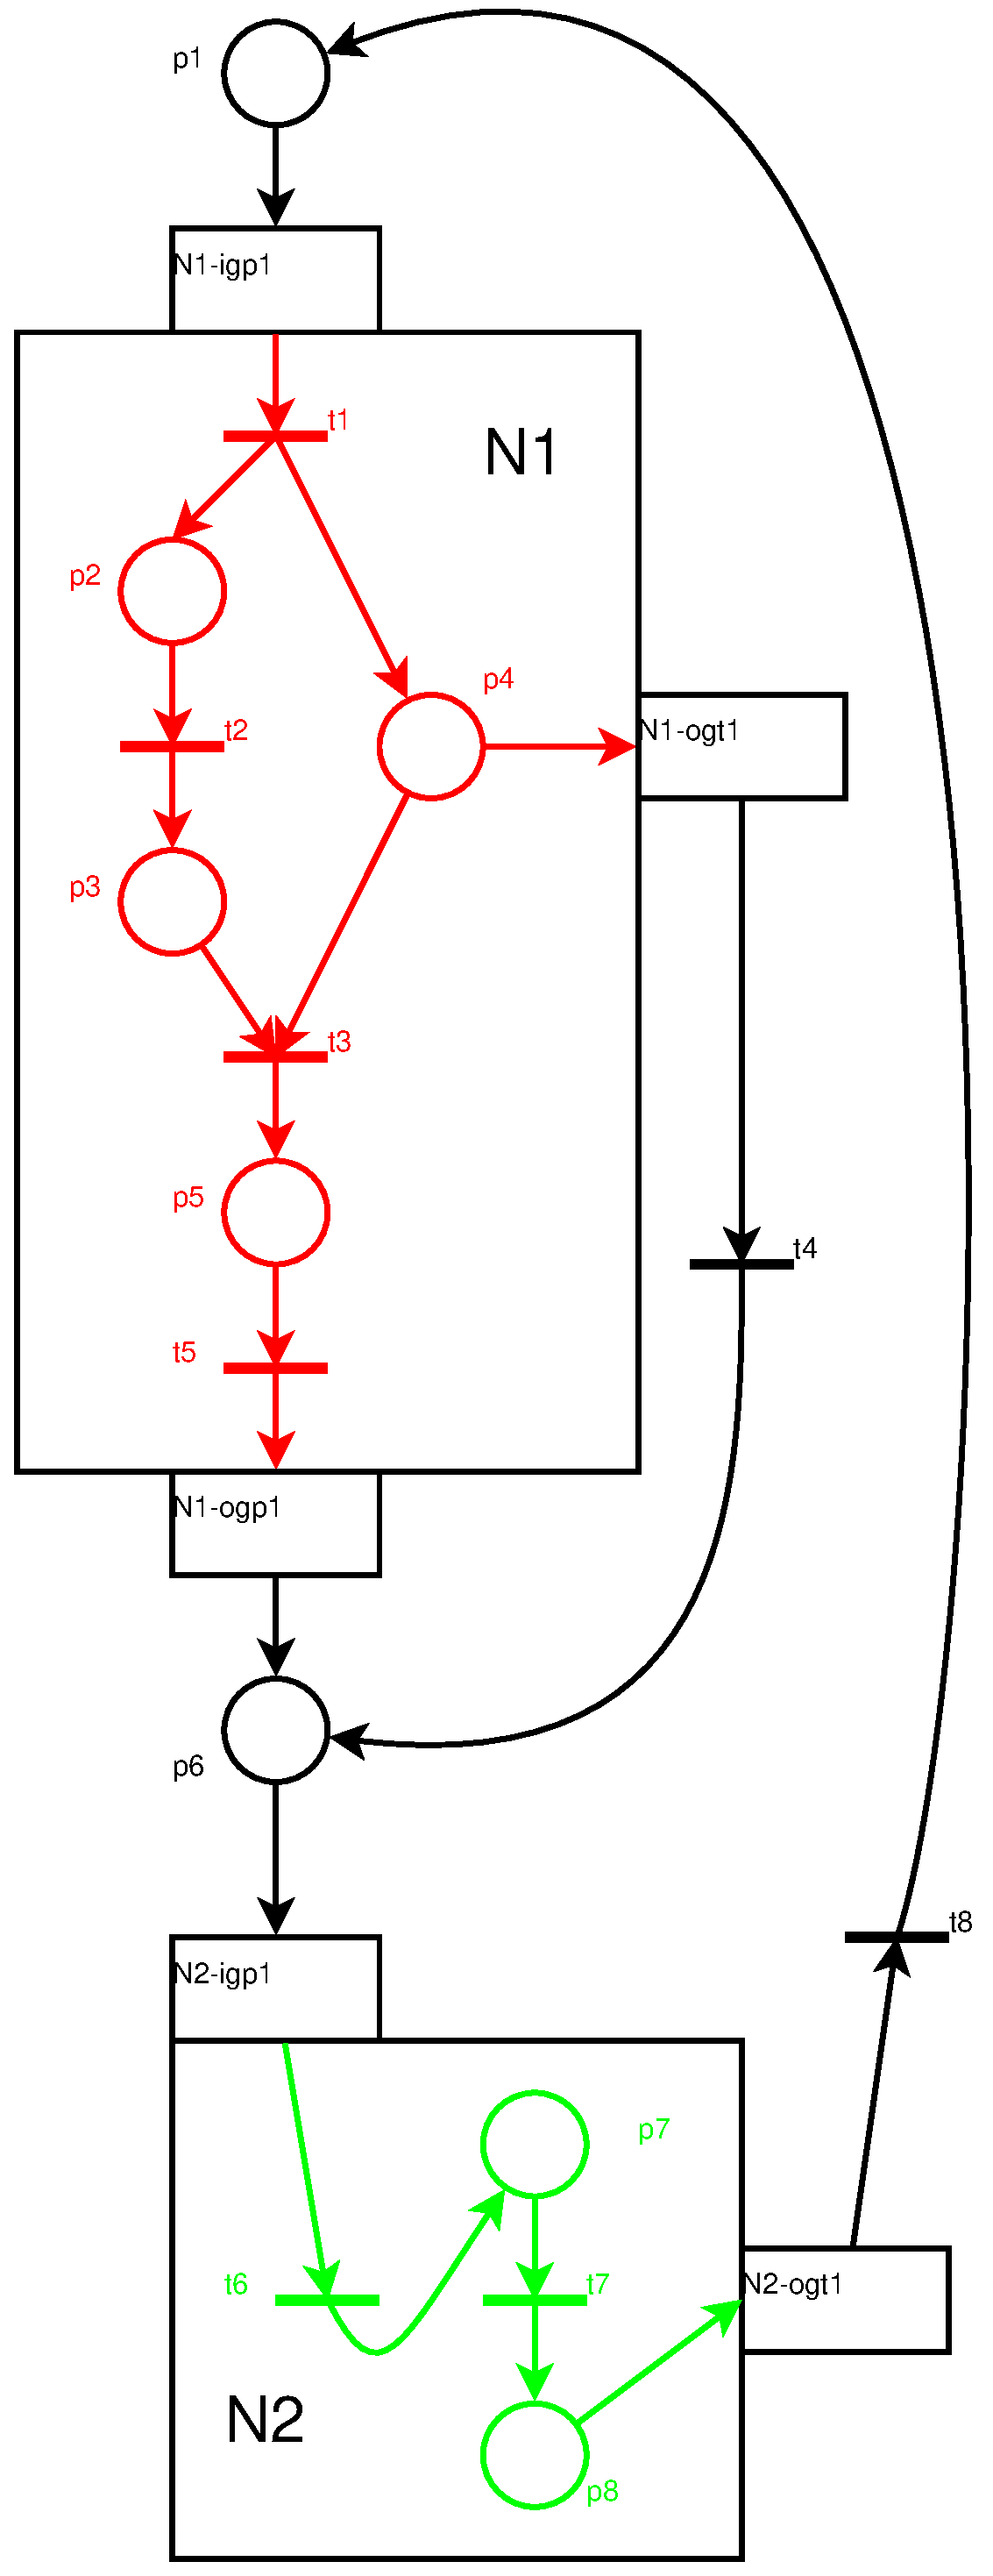
\includegraphics[width=0.35\textwidth]{Figures/PNML-Latorre_1_subnets_interfaces.eps}
\]

and this is the XML content with the signature of all the subnets:

\begin{lstlisting}[basicstyle=\ttfamily\tiny]
<?xml version="1.0" encoding="UTF-8"?>
<pnml xmlns="http://www.pnml.org/version-2009/grammar/pnml">
  <net id="latorre1" type="http://www.pnml.org/version-2009/grammar/ptnet">
    <page id="page1">
      <subnet id="N1">
        <interface id="N1-interface">
          <gate action="input" id="N1-igp1" type="place"/>
          <gate action="output" id="N1-ogt1" type="transition"/>
          <gate action="output" id="N1-ogp1" type="place"/>
        </interface>
        <content id="N1_content">
          <place id="p2"/>
          <place id="p3"/>
          <place id="p4"/>
          <place id="p5"/>
          <transition id="t1"/>
          <transition id="t2"/>
          <transition id="t3"/>
          <transition id="t5"/>
          <arc id="a2" source="t1" target="p2"/>
          <arc id="a3" source="p2" target="t2"/>
          <arc id="a4" source="t2" target="p3"/>
          <arc id="a5" source="t1" target="p4"/>
          <arc id="a6" source="p3" target="t3"/>
          <arc id="a8" source="p4" target="t3"/>
          <arc id="a9" source="t3" target="p5"/>
          <arc id="a10" source="p5" target="t5"/>
          <arc id="N1-a1" source="N1-igp1" target="t1"/>
          <arc id="N1-a7" source="p4" target="N1-ogt1"/>
          <arc id="N1-a11" source="t5" target="N1-ogp1"/>
        </content>
      </subnet>
      <subnet id="N2">
        <interface id="N2-interface">
          <gate action="input" id="N2-igp1" type="place"/>
          <gate action="output" id="N2-ogt1" type="transition"/>
        </interface>
        <content id="N2_content">
          <place id="p7"/>
          <place id="p8"/>
          <transition id="t6"/>
          <transition id="t7"/>
          <arc id="a13" source="t6" target="p7"/>
          <arc id="a14" source="p7" target="t7"/>
          <arc id="a15" source="t7" target="p8"/>
          <arc id="N2-a12" source="N2-igp1" target="t6"/>
          <arc id="N2-a16" source="p8" target="N2-ogt1"/>
        </content>
      </subnet>
      <place id="p1"/>
      <place id="p6"/>
      <transition id="t4"/>
      <transition id="t8"/>
      <arc id="a1" source="p1" target="N1-igp1"/>
      <arc id="a7" source="N1-ogt1" target="t4"/>
      <arc id="a11" source="N1-ogp1" target="p6"/>
      <arc id="a12" source="p6" target="N2-igp1"/>
      <arc id="a16" source="N2-ogt1" target="t8"/>
      <arc id="a17" source="t8" target="p1"/>
      <arc id="a18" source="t4" target="p6"/>
    </page>
  </net>
  <ds:Signature xmlns:ds="http://www.w3.org/2000/09/xmldsig#">
    <ds:SignedInfo>
      <ds:CanonicalizationMethod Algorithm="http://www.w3.org/TR/2001/REC-xml-c14n-20010315"/>
      <ds:SignatureMethod Algorithm="http://www.w3.org/2000/09/xmldsig#rsa-sha1"/>
      <ds:Reference URI="">
        <ds:Transforms>
          <ds:Transform Algorithm="http://www.w3.org/2000/09/xmldsig#enveloped-signature"/>
          <ds:Transform Algorithm="http://www.w3.org/TR/2001/REC-xml-c14n-20010315#WithComments"/>
          <ds:Transform Algorithm="http://www.w3.org/2002/06/xmldsig-filter2">
            <dsig-xpath:XPath xmlns:dsig-xpath="http://www.w3.org/2002/06/xmldsig-filter2"
                Filter="intersect">/pnml/net/page/subnet</dsig-xpath:XPath>
          </ds:Transform>
        </ds:Transforms>
        <ds:DigestMethod Algorithm="http://www.w3.org/2000/09/xmldsig#sha1"/>
        <ds:DigestValue>2jmj7l5rSw0yVb/vlWAYkK/YBwk=</ds:DigestValue>
      </ds:Reference>
    </ds:SignedInfo>
    <ds:SignatureValue>
      PIwJ414XUFjfd5IYFcJBKeCmYJfanN7Wcus5F5PJRl1yMGVcfeocqQv1nTAn86pQW4NxhYrXEEnD
      zO5Dic/aKC/jt8zgnCZ81DVLCnJLmtc61ltKezEs0ekE6A9PsRjP0DusqtVKL4C2miiFiPsL3enn
      rXBk3ZPYpLcXZw5q/js=
    </ds:SignatureValue>
    <ds:KeyInfo>
      <ds:X509Data>
        <ds:X509Certificate>
          MIICgTCCAeqgAwIBAgIETfh4CTANBgkqhkiG9w0BAQUFADCBhDELMAkGA1UEBhMCRVMxETAPBgNV
          BAgTCExBIFJJT0pBMREwDwYDVQQHDAhMT0dST8KlTzEgMB4GA1UEChMXVU5JVkVSU0lEQUQgREUg
          TEEgUklPSkExDDAKBgNVBAsTA1BGQzEfMB0GA1UEAwwWScKlSUdPIExFw6BOIFNBTUFOSUVHTzAe
          Fw0xMTA2MTUwOTE0NDlaFw0xMTA5MTMwOTE0NDlaMIGEMQswCQYDVQQGEwJFUzERMA8GA1UECBMI
          TEEgUklPSkExETAPBgNVBAcMCExPR1JPwqVPMSAwHgYDVQQKExdVTklWRVJTSURBRCBERSBMQSBS
          SU9KQTEMMAoGA1UECxMDUEZDMR8wHQYDVQQDDBZJwqVJR08gTEXDoE4gU0FNQU5JRUdPMIGfMA0G
          CSqGSIb3DQEBAQUAA4GNADCBiQKBgQChePFNVCIfphFlyXQ9BysiR5BfXIuv3AnAK80Fuw4tTFwC
          nVUjJeGnkUYQO32oUu+fEBK8WsEqjeH8A7zrHTRQjfYZWyuGWrM8gJXOa/P0MROPm/c/H8b5a6Nx
          1/+zLwR0tYkqLI2xqDOFII2RwK5L2yGeV4T4y8i3h1U0OFTSEwIDAQABMA0GCSqGSIb3DQEBBQUA
          A4GBAIDOvAAdOCaTpy+83bGB2KmngMJrNxxWDpAi5LGFrN8iCShmbTpIeIbYBUAaBpZtdhOnhq4n
          wD5QOENSFipQcdH5GEpPM9Rquy6xMwfda9EU5UfOSEmbk4fK2vaIOVjynpQsJ9P99enO2smQlyvw
          /hBa7Xacz6qDut8ghUeuV5Js
        </ds:X509Certificate>
      </ds:X509Data>
      <ds:KeyValue>
        <ds:RSAKeyValue>
          <ds:Modulus>
            oXjxTVQiH6YRZcl0PQcrIkeQX1yLr9wJwCvNBbsOLUxcAp1VIyXhp5FGEDt9qFLvnxASvFrBKo3h
            /AO86x00UI32GVsrhlqzPICVzmvz9DETj5v3Px/G+Wujcdf/sy8EdLWJKiyNsagzhSCNkcCuS9sh
            nleE+MvIt4dVNDhU0hM=
          </ds:Modulus>
          <ds:Exponent>AQAB</ds:Exponent>
        </ds:RSAKeyValue>
      </ds:KeyValue>
    </ds:KeyInfo>
  </ds:Signature>
</pnml>
\end{lstlisting}


%----------------------------------------------------------------------------------------
%       SECURITY: Complete security
%----------------------------------------------------------------------------------------
\section{Complete security}

In this section I am going to explain several important questions.
Until now, I have described the two security operation separately: hiding
and signing. I want some parts to be hidden and other parts to be signed.
But, what would happen if I want to hide and sign the same parts?
In this case, the result is different depending on the order selected. Let's
see the differences.

Suppose first cipher and then sign. If this order is applied, the cipher has no problem, but the sign has a obvious but important detail: the signed content is
encrypted itself. What does it mean? Well, you don't see what you are signing. The implications are simple: you don't know exactly what you are signing. This order is useful in order to guarantee the integrity, but you have to be sure that what you are signing is exactly what you want.

The other order is: first signing and then ciphering. In this case, signing
has no problem. The special characteristic is the ciphering. As explained
before in this chapter, after signing, appears a new tag \texttt{<Signature>}
appended to the original content. Then, if I encrypt the signed content,
this tag is still visible but the signature cannot be verified, because the
encrypting process replace the original content, so there is a modification
of the signed data and it is detected by the signature, avoiding a correct
verification of it.

The selected order depends on the responsible of each part. Anyway, there
is a W3C recommendation that describes a XMLSignature decryption transform \cite{XMLSIG-w3.org/xmlenc-decrypt} that permits to differentiate between ciphered content that were encrypted \emph{before} signing (and must not be decrypted) and ciphered content that were encrypted \emph{after} signing (and must be decrypted). So the XML applications are able to interpret the correct
way to validate the signature. As it is a particular case of configuration, and my intention is explain the general guidelines, I am not going to explain it here. Again, the responsible of the net/subnet is who has to decide the concrete configuration, but maintaining the general rules that I explain in this thesis.

%----------------------------------------------------------------------------------------
%       SECURITY: Conclusions
%----------------------------------------------------------------------------------------
\section{Conclusions}

As we have seen, one of the applications of subnetting Petri nets and represent
them in PNML is that I can apply standard processes based on XML. In this
case, once defined and represented a subnet in PNML, I have applied XMLEncryption in order to hide the internal structure of the subnet and XMLSignature for
signing the subnet. 

The use of standard and widely extended technologies like XMLEncryption and
XMLSignature enables that everybody has access to them, so the processes
explained here are perfectly usable. 

One important conclusion in the encryption section is that several subnets in the same net can be ciphered with different
options. This is used, for example, for  one receiver
to decrypt the subnet addressed to him but no other one.

Other important
use is that with a PNML file with encrypted subnets, I can replace one ciphered subnet by other ciphered subnet without the necessity of decrypt any of them: we can work with encrypted subnets if the interfaces are the same. 
With the explained in this chapter, the privacy of parts of a Petri net is guarantied.


In XMLSignature,   integrity, authentication and non repudiation is assured.
A big difference with XMLEncryption is that the signature is attached to
the original file, instead of replace part of the net. In this case I have used enveloped signature, but if we use the
detached way, the signature is in other file, separating signature and signed content. In signature it makes no sense replace one signature by another,
but we can have as many signatures as we want, including different signatures of the same contents.

  
Using both technologies XMLEncryption and XMLSignature together we can reach
very high security levels, but we have to be careful with the order of the processes, because depending on the selected order, the acquired properties will be different.

The last conclusion, but very important one is that the responsible of the net has to choose the concrete configurations of XMLEncryption and XMLSignature, the transforms and the order of the actions in order to achieve his particular objectives. 
